% ============================================================================
% JEDC 投稿核心章节（英文稿）：AGI 转型的平稳过渡动力学
% 交付：LaTeX 源文件（elsarticle 文档类，含 frontmatter/摘要/关键词/JEL 与嵌入图）。
% 依据：JEDC_model_formalization.md（定理 1–6）+ JEDC_calibration.md（修正校准）
%       + JEDC_literature_contrast.md（增量声明）。数值为修正校准重跑（eta=0.40, mu_TM=0.50）。
% 说明：已通过静态结构检查，并在云端 TeX Live（elsarticle + lmodern + T1 + microtype）编译验证。
% ============================================================================
\documentclass[review,12pt]{elsarticle}
\usepackage[margin=1in]{geometry}
\usepackage{amsmath,amssymb,amsthm}
\usepackage{booktabs,array}
\usepackage{graphicx}
\usepackage[utf8]{inputenc}
\usepackage[T1]{fontenc}
\usepackage{lmodern}
\usepackage{xurl}
\usepackage{microtype}
\graphicspath{{figures/}}

\theoremstyle{plain}
\newtheorem{theorem}{Theorem}
\newtheorem{corollary}[theorem]{Corollary}
\newtheorem{proposition}[theorem]{Proposition}
\newtheorem{lemma}[theorem]{Lemma}
\theoremstyle{definition}
\newtheorem{definition}[theorem]{Definition}
\theoremstyle{remark}
\newtheorem{remark}[theorem]{Remark}

\newcommand{\dd}{\,\mathrm{d}}
\newcommand{\barL}{\bar{L}}
\newcommand{\bm}{\boldsymbol}

\begin{document}
\begin{frontmatter}

\title{Anatomy of a Smooth Transition: A Task-Based Macroeconomic Model of AGI Displacement with Fiscal and Social Safety Nets}

\author[addr1]{DUAN Fang\corref{cor1}}
\ead{duan.fang@hqu.edu.cn}
\address[addr1]{Huaqiao University, School of Information Science and Engineering, Xiamen, China}
\cortext[cor1]{Corresponding author.}

\begin{abstract}
Artificial general intelligence (AGI) differs from automation in that it enters the creation of new tasks itself, so the engine that historically reinstated displaced labor may collapse endogenously. We build a task-based model with two-layer task structure in which the human reinstatement rate declines as AI capability advances, plus nominal rigidity, the zero lower bound and debt-deflation, capital-tax financing of workfare and transfers, and an independent social-instability channel. The high-employment equilibrium is lost through a boundary equilibrium bifurcation of the piecewise-smooth fast subsystem; we derive a closed-form critical reinstatement rate, make it endogenous to workfare and retraining, and characterize with geometric singular perturbation theory the finite-rate lag between slow policy and fast employment. Three magnitudes are anchored to U.S. data; the rest are declared settings. Under these settings, the loss-minimizing policy on the reported grid is a workfare-dominant corner financed by a minimal capital tax, whereas no-policy and pure-transfer regimes are infeasible. The minimizer is grid-dependent rather than identified; we report the corner retaining a buffer. At the baseline frontier growth $g_A=0.010$, consumption stays above the floor $C^{min}=0.30$ with $\min_t C_t=0.309$, but at $g_A=0.05$ the floor is already breached ($\min_tC_t=0.283$) and the path crashes, whereas fiscal parameters are nearly inert. Frontier-growth shocks ($\sigma$ up to $0.03$) leave the reported corner intact ($6$ of $200$ paths crash) but violate the buffer-free minimizer ($143$ of $200$). The model-implied message: a smooth transition requires a financed buffer whose sufficiency is conditional on frontier speed.
\vspace{6pt}\noindent\textit{JEL classification:} E24, E31, E62, J64, O33.
\end{abstract}

\begin{keyword}
Artificial general intelligence \sep Task-based model \sep Boundary equilibrium bifurcation \sep Geometric singular perturbation theory \sep Public employment \sep Labor share
\end{keyword}

\end{frontmatter}

% ============================================================================
\section{Introduction}
% ============================================================================
Artificial general intelligence (AGI) and large-scale automation portend a fundamental reallocation of work. Task-based analyses of recent automation show that new-task creation has historically reinstated labor displaced by machinery (Acemoglu--Restrepo)~\cite{AR2018}, but the AGI setting is different in kind: AGI participates in \emph{new-task creation itself}, so the reinstatement engine may collapse endogenously. The recent AGI macroeconomics literature splits into two poles. On the \emph{supply side}, Restrepo (2025)~\cite{Restrepo2025} and Korinek--Suh (2024)~\cite{KS2024} characterize conditions under which automation collapses wages: when the complexity of tasks humans can perform is bounded and full automation is reached, or when automation outruns capital accumulation. On the \emph{demand side}, Fornaro--Wolf (2026)~\cite{FW2026} stress that automation shifts income from high-MPC workers to savers, weakening aggregate demand and lowering the natural rate. Yet these two poles remain disconnected, and neither connects wage collapse to the \emph{transitional fiscal policy} needed to sustain demand while the labor share vanishes.

This paper proposes a task-based macroeconomic model that closes these gaps in a single, numerically solvable switching system. Its ingredients are: a two-layer task model (production and creative tasks) in which the reinstatement engine collapses endogenously as AGI participation $\kappa_N^{AI}$ dominates human new-task creation; a demand side with nominal rigidity, the zero lower bound, and debt-deflation; a fiscal closure in which a capital tax finances workfare (public employment) and transfers under a balanced-budget constraint; and a social-instability channel independent of economic deflation, in which a large purely-relief population generates social pressure. The central methodological challenge is that feasibility here is a question not about a single equilibrium but about whether the high-employment branch still exists: in a piecewise-smooth switching system with a slow fiscal layer and a fast employment layer, no local linearization can answer it, so the transition has to be posed as a bifurcation problem.

Our analytical results are six. We prove that reinstatement collapse drives the labor share monotonically to zero with no self-correcting mechanism, and that skill-retention value is proportional to the reinstatement rate $\omega$, vanishing as $\omega\to0$ (Theorem~\ref{thm1}). We upgrade Fornaro--Wolf's demand shortfall into an explicit, decidable deflationary spiral (Theorem~\ref{thm2}), cascading the wage-collapse source into crash dynamics. We establish the existence of a smooth-transition region and a Laffer interior capital tax $\tau^*$ (Propositions~\ref{prop3a}--\ref{prop3b}), and show public employment strictly dominates transfers within a given budget because $1>\mu_{TM}$ (Proposition~\ref{prop4}). We prove that workfare has a structural protective advantage over pure UBI against social-instability risk (Proposition~\ref{prop5}), and establish a robustness ceiling for the entire buffer family: beyond a critical shock intensity, no combination of workfare and transfers can prevent an economic crash, so strong shocks require supply-side structural measures (Proposition~\ref{prop6}).

Beyond these switching-system results, we develop an analytic bifurcation theory that makes the collapse mechanism itself tractable (Section~\ref{sec:bifurcation}). Deriving the fast subsystem directly from the model, we show that its vector field is quadratic and that the high-employment branch is lost through a boundary equilibrium bifurcation at the piecewise-smooth switching manifold; we derive a closed-form critical reinstatement rate and then make that rate endogenous to public employment, workfare and retraining, so policy can move the system across the bifurcation, and use geometric singular perturbation theory to characterize the finite-rate lag of the fast employment variable.

We anchor three magnitudes to U.S. data---the consumption floor, the transfer MPC $\mu_{TM}=0.50$, and the workfare wage ratio---set the remaining entries by explicit convention, including the capital-tax growth inhibition $\eta=0.40$, and run the full battery of experiments under a unified engine (Section~\ref{sec:calibration}). The six analytical results P1--P6 are reproduced within the reported grid; the minimum-loss point on the grid is a corner solution (workfare-dominant, transfers closed, minimal sufficient capital tax) whose coordinates are grid-dependent rather than identified, and, within this calibrated model at the baseline frontier growth $g_A=0.010$, no-policy and pure-transfer regimes are infeasible because they violate the financing constraint, while the smooth outcome itself is conditional on $g_A$: it is lost once $g_A$ reaches $0.05$ (Section~\ref{sec:calibration}). No parameter is estimated here, and none of the critical values is presented as one: the reinstatement rate at which the high-employment branch is lost, and the interior workfare share $p_E^*$, are dimensionless outputs of the calibrated model, so the paper claims structural insight rather than external identification. The central message, read as a model-implied rather than a universal claim, is that a smooth AGI transition \emph{requires a policy buffer, and that buffer must be financed}.

The remainder of the paper is organized as follows. Section~\ref{sec:model} lays out the model. Section~\ref{sec:main-results} derives the analytical propositions. Section~\ref{sec:bifurcation} develops the analytic boundary equilibrium bifurcation theory. Section~\ref{sec:calibration} presents the calibration and the numerical evidence. Section~\ref{sec:literature} situates the contributions relative to the literature, and Section~\ref{sec:conclusion} concludes.

% ============================================================================
\section{The Model}
\label{sec:model}
% ============================================================================

\subsection{Environment}
Discrete time $t=0,1,\dots,T$. A continuum of labor $L^S=\barL=1$ is supplied inelastically and the wage is the num\'eraire, $w=1$. Three agents populate the economy: firms that produce with a task technology; a government that taxes capital income and runs transfers / public employment; and households that consume, save, and supply labor. This is a deterministic switching system of aggregate difference equations (neither a DSGE nor an agent-based model) with no stochastic shocks along the baseline path (Table~\ref{tab:shock} adds a frontier-growth shock ensemble as a robustness check); all state variables are deterministic time-indexed arrays.

The state variables are the automation threshold $I_t$, the upper bound of new tasks $N_t$, the labor-task share $n_t\equiv N_t-I_t$, employment $L_t^D$, the labor share of employment $s_t\equiv L_t^D/\barL$ (called the labor share throughout; it equals the wage-bill share $w_tL_t^D/Y_t$ only while $w\barL=Y_t$), the price level $P_t$, nominal debt $D_t$, real debt $b_t\equiv D_t/P_t$, a skill stock $\sigma_t$, and a social-pressure index $\varsigma_t$.

\subsection{Technology: a two-layer task model with an endogenously collapsing reinstatement engine}
\label{sec:technology}
We extend the Acemoglu--Restrepo task framework to two layers: a production-task layer and a creative-task layer that can itself be automated.

\textbf{Automation (displacement) frontier.}
\begin{equation}
\dd I_t=\kappa_I\,A_t,\qquad A_t=A_0(1+g_A)^t.
\end{equation}

\textbf{Reinstatement (new-task creation) engine.}
\begin{equation}
\dd N_t=\kappa_N^{h}\,S_t^h+\kappa_N^{AI}\,A_t\,M_0,
\qquad S_t^h=S_0\max\{0,\,1-\lambda_h\,I_{t-1}/N_{t-1}\},
\end{equation}
where $S_t^h$ is creative labor still performed by humans and $\kappa_N^{AI}$ governs AGI participation in new-task creation. The reinstatement engine \emph{collapses endogenously}: when $\kappa_N^{AI}\gg\kappa_N^h$, the locus of new-task creation switches from humans to compute.

\textbf{Net labor-task expansion (reinstatement minus displacement) with a skill channel.}
\begin{equation}
\dd n_t=\omega\,\big(\dd N_t\big)\,\sigma_{t-1}-\dd I_t,\qquad
n_t=\max\{0,\,n_{t-1}+\dd n_t\},
\end{equation}
where $\omega\in(0,1]$ is the \emph{reinstatement rate}, the share of new tasks accruing to labor; held exogenous here and endogenized in Section~\ref{sec:bifurcation}, and $\sigma_{t-1}$ is the skill stock. \textbf{Key modelling choice}: the value of skills is proportional to $\omega$. When $\omega\to0$ (AGI takes over new-task creation, so new tasks no longer accrue to labor), skills have no economic return even at arbitrarily high levels. This mechanizes Restrepo's (2025) proposition that skills no longer determine wages.

\textbf{Employment and the labor share.}
\begin{equation}
L_t^D=\barL\cdot\min\{1,\;\max\{0,\,n_t/N_t\}\},\qquad s_t=L_t^D/\barL.
\end{equation}

\textbf{Skill stock (retraining vs.\ public employment).}
\begin{equation}
\sigma_t=\sigma_{t-1}\Big(1-\delta_\sigma\,\tfrac{U_t^{rem}}{\barL}\,\big(1-\rho_{ret}\,\beta_{ret}\big)\Big),\qquad
\sigma_t\ge\underline{\sigma}=0.30.
\end{equation}
Skills are preserved only by retraining $\rho_{ret}\in[0,1]$; $\beta_{ret}\in[0,1]$ scales how effectively retraining offsets skill decay, and public employment (workfare) does not preserve skills.

\textbf{Output.}
\begin{equation}
Y_t=(1+g_{eff})^t\,\big(1+g_{disp}\,\delta_{disp}\big),\qquad
g_{eff}=g_G(1-\eta\tau),\qquad \delta_{disp}=(I_t-I_0)/N_0,
\end{equation}
where $g_{eff}$ embeds the Laffer-style supply-side cost of the capital tax $\tau$.

\textbf{Capital income (tax base) and taxation.}
\begin{equation}
\Pi_t=\max\{0,\;Y_t-w_{t-1}L_t^D\},\qquad \text{tax}_t=\tau\,\Pi_t.
\end{equation}

\subsection{Demand side: nominal rigidity, the zero lower bound, and debt-deflation}
\textbf{Wage rule} (empirical, not a market-clearing condition):
\begin{equation}
w_t=\max\{\underline{w},\;w_{t-1}\,(1+g_W-\lambda_w\,u_t)\},\qquad u_t=1-s_t.
\end{equation}

\textbf{Inflation from the consumption gap.}
\begin{equation}
\pi_t=\max\{\pi^{lb},\;\gamma_p\,(C_{t-1}/C^{fe}-1)\},\qquad P_t=P_{t-1}(1+\pi_t),
\qquad C^{fe}\equiv w\,\barL.
\end{equation}

\textbf{Nominal interest and the zero lower bound (ZLB).}
\begin{equation}
i_t=\max\{0,\;r_n+\pi_t\},\qquad r_t^d=i_t-\pi_t.
\end{equation}

\textbf{Debt-deflation.}
\begin{equation}
D_t=D_{t-1}(1+i_t)+\max\{0,\,C^{fe}-C_{t-1}\}\,\theta,\qquad b_t=D_t/P_t.
\end{equation}

\textbf{Consumption.}
\begin{equation}
C_t=w_tL_t^D+w^P E_t^P+\mu_{TM}\,TM_t
-\zeta\max\{0,\,b_t-\bar b\}-\mu_d\max\{0,\,r_t^d\},\qquad C_t\ge0,
\end{equation}
with $w^P E_t^P$ public-employment wages and $\mu_{TM}TM_t$ transfers subject to a leakage $\mu_{TM}\in(0,1)$. In the numerical implementation the excess real debt $b_t-\bar b$ is capped at $0.8$, so the drag term is bounded above by $0.8\zeta$, to avoid over-determining the Euler cut-off. The cap is a numerical safeguard and binds only on paths that have already breached the floor, so the simulated crash is generated by the employment and consumption channel rather than by the debt-drag term; the unbounded-divergence chain in Theorem~\ref{thm2} describes the analytical limit without the cap.

\subsection{Fiscal closure: the transition financing gap}
\textbf{Policy response (with delay $d$):}
\begin{equation}
\phi_t=\min\{\phi^{\max},\;\phi^{base}+\rho_{resp}\,u_{t-d}\}.
\end{equation}

\textbf{Planned spending.}
\begin{equation}
E_t^{plan}=w^P E_t^P+\phi_t\,w\,U_t^{rem},\qquad
E_t^P=\min\{p_E\,u_t\barL,\;u_t\barL\},\qquad U_t^{rem}=u_t\barL-E_t^P.
\end{equation}

\textbf{Balanced budget / fiscal feasibility:}
\begin{equation}
\text{actual spending}=\min\{E_t^{plan},\;\text{tax}_{t-1}\},\quad
\text{shortfall}\Rightarrow \text{proportional scaling }\rho=\text{tax}_{t-1}/E_t^{plan}.
\end{equation}
Appropriations in period $t$ are funded by taxes already collected in $t-1$: the government budgets against last period's realized revenue, so the fiscal constraint uses $\text{tax}_{t-1}$ rather than the current-period tax. A financing-constraint collapse occurs when the tax base is too small to fund the floor, consumption falls below the subsistence level, and the economy crashes.

\subsection{Social instability (an independent failure channel)}
\label{sec:social-instability}
\begin{equation}
\varsigma_t=\alpha_s\,(U_t^{rem}/\barL).
\end{equation}
The larger the purely-relief population (smaller $p_E$), the larger the social pressure. If $\varsigma_t>\varsigma^{th}$ for $J$ consecutive periods, a \emph{social-instability collapse} occurs. Public employment converts relief recipients into dignified jobs, reducing pressure. This is the mechanism behind ``workfare $>$ pure UBI.'' The cutoff values $\varsigma^{th}=0.50$, the persistence requirement $J=10$, and the coefficient $\alpha_s=0.60$ are reduced-form model choices rather than externally estimated quantities: $\varsigma^{th}$ has no direct external anchor, while $\alpha_s$ and $J$ are only partially anchored (Section~\ref{sec:social-anchor}). The workfare-over-UBI ranking is therefore conditional on these cutoffs. Section~\ref{sec:calibration} reports a systematic sensitivity sweep that quantifies how far each cutoff must move before the corner policy triggers this channel, and Section~\ref{sec:social-anchor} bounds the channel against the empirical ranges.

\subsection{Equilibrium and the steady state}
\textbf{Smooth path.} Given parameters and policy $(\tau,p_E,\phi^{\max},\omega,\dots)$, the system attains a \emph{smooth transition} if, in finite time: (i) $s_t<s^{th}\equiv0.05$ in finite time (the employment share falls below the absorbing value); (ii) $\min_t C_t\ge C^{min}\equiv q\,w\barL$; (iii) inflation is not persistently negative; (iv) $\varsigma_t$ does not exceed the threshold persistently; (v) the financing constraint is not violated; (vi) $b_t$ does not diverge. Otherwise the outcome is an \emph{economic collapse} (deflationary spiral / debt / consumption below floor), a \emph{social-instability collapse}, or \emph{not-reached}. In our model the outcome is gated by (ii) the consumption floor and (iv) the social threshold. The deflationary spiral and debt divergence of Theorem~\ref{thm2} are the mechanism through which (ii) is breached once the wage bill collapses and the gap is left unabsorbed, so (ii) nests the spiral rather than competing with it. The labels are ex-post classifications over the full $T=80$ simulation, not absorbing-state interruptions.

% ============================================================================
\section{Main Results: Analytical Propositions}
\label{sec:main-results}
% ============================================================================
\subsection{Reinstatement collapse drives the labor share monotonically to zero}
\begin{theorem}[Reinstatement Collapse]
\label{thm1}
Assume (A1) $\kappa_I>0$, $A_t=A_0(1+g_A)^t$, $A_0>0$ (strictly monotone displacement frontier); (A2) there exists $\overline{\dd N}<\infty$ with $\dd N_t\le\overline{\dd N}$, and $\sigma_{t-1}\in[\underline{\sigma},1]$. If for all $t\ge t_0$,
\[
\omega\,\sigma_{t-1}\,\dd N_t<\dd I_t=\kappa_I A_t,
\]
then $n_t$ is strictly decreasing, there is a finite $T^*$ with $n_{T^*}=0$, and $s_t=0$ for all $t\ge T^*$.
\end{theorem}
\begin{proof}
(i) By the premise $\dd n_t=\omega\dd N_t\sigma_{t-1}-\dd I_t<0$, so $n_t$ is strictly decreasing while positive.
(ii) Uniform negative drift. By A1, $A_t=A_0(1+g_A)^t$ grows exponentially; by A2, $\dd N_t\le\overline{\dd N}$ and $\sigma_{t-1}\le1$. Define
\[
t_1=\max\!\left\{0,\ \left\lceil\frac{\ln(2\omega\overline{\dd N}/(\kappa_I A_0))}{\ln(1+g_A)}\right\rceil\right\}.
\]
Then $\kappa_I A_{t_1}\ge2\omega\overline{\dd N}$, and for all $t\ge\max\{t_0,t_1\}$,
\[
\dd n_t=\omega\sigma_{t-1}\dd N_t-\kappa_I A_t\le\omega\overline{\dd N}-\kappa_I A_{t_1}\le-\omega\overline{\dd N}<0.
\]
Hence from $t_1$ onward $n_t$ falls by at least $\omega\overline{\dd N}>0$ per period; starting from $n_{t_1}\le N_0$, it reaches zero in at most $N_0/(\omega\overline{\dd N})$ periods. The interval up to $t_1$ is finite, and the premise already gives $\dd n_t<0$ over it. Hence $T^*<\infty$ and $n_{T^*}=0$.
(iii) Once $n=0$, $L_t^D=0$ and $s_t=0$; $\max\{0,\cdot\}$ keeps $s_t=0$ thereafter. $\square$
\end{proof}

\begin{corollary}[Zero-reinstatement limit, $\omega\to0$]
\label{cor1}
Since $\omega\,\sigma\,\dd N_t\le\omega\,\overline{\dd N}\to0<\kappa_I A_t$, the premise holds for large $t$. Hence as $\omega\to0$ (AGI takes over new-task creation), the labor share vanishes monotonically with \emph{no self-correcting mechanism}.
\end{corollary}

\begin{remark}
This is consistent with ``skills no longer determine wages'' (Restrepo, 2025), but here the reinstatement collapse is \emph{endogenous}, driven by $\kappa_N^{AI}/\kappa_N^h$ and $\omega$, not an exogenous bounded-complexity terminal state.
\end{remark}

\subsection{The deflationary spiral}
\begin{theorem}[Deflationary Spiral]
\label{thm2}
Assume (B1) there exist $t_0$ and $\varepsilon>0$ such that, for all $t\ge t_0$,
\[
C_{t-1}\le\big(1+\pi^{lb}/\gamma_p-\varepsilon\big)C^{fe}\approx0.867\,C^{fe},
\]
so that the inflation floor binds (calibrated $\pi^{lb}=-0.02,\gamma_p=0.15$);
(B2) $r_n<-\pi^{lb}$; (B3) $\zeta>0$ and $\bar b<\infty$; (B4) income $W_t\equiv w_tL_t^D+w^P E_t^P+\mu_{TM}TM_t$ satisfies $W_t\le C^{fe}-\varepsilon$, $\varepsilon>0$. Then:
(i) $\pi_t=\pi^{lb}<0$, $i_t=0$, $r_t^d=-\pi^{lb}>0$ for all $t\ge t_0$;
(ii) $D_t$ is nondecreasing and $b_t$ strictly increasing with no upper bound;
(iii) there is a finite $T$ with $b_T>\bar b$, after which the debt-drag term strictly increases;
(iv) hence the upper bound on $C_t$ declines without bound, so $C_t$ eventually satisfies $C_T<C^{min}$, triggering the economic-crash channel.
\end{theorem}
\begin{proof}
(i) $C_t<C^{fe}\Rightarrow\pi_t=\pi^{lb}$ (B1); $i_t=0$ (B2); $r_t^d=0-\pi^{lb}>0$.
(ii) With $i_t=0$, $D_t=D_{t-1}+\theta(C^{fe}-C_{t-1})$ is nondecreasing; $P_t=P_{t_0}(1+\pi^{lb})^{t-t_0}$ falls; so $b_t=D_t/P_t$ strictly increases and, as $D_t\to\infty$, $P_t\to0$, is unbounded.
(iii) As $b_t\to\infty$, a finite $T$ with $b_T>\bar b$ exists; afterwards $\zeta(b_t-\bar b)$ strictly increases.
(iv) For $t\ge T$, $C_t=W_t-\zeta(b_t-\bar b)-\mu_d r_t^d$. By B4, $W_t\le C^{fe}-\varepsilon$; since the debt term diverges, $C_t$ is bounded above by $C^{fe}-\varepsilon-\zeta(b_t-\bar b)-\mu_d r_t^d\to-\infty$ (monotonicity of $W_t$ is not required); hence $C_t$ breaches $C^{min}$ in finite time. $\square$
\end{proof}

\begin{remark}
The two conditions cascade: Theorem~\ref{thm1} supplies the source of the gap (wage collapse $wL^D\to0$), and Theorem~\ref{thm2} characterizes its crash dynamics (ZLB activated $r_n<-\pi^{lb}$, gap not absorbed by fiscal transfers). This upgrades Fornaro--Wolf's ``demand shortfall'' into an explicit, decidable failure channel.
\end{remark}

\subsection{Existence of a smooth region and the Laffer interior solution}
\begin{proposition}[Existence]
\label{prop3a}
If for all $t$: (C1) $\text{tax}_{t-1}\ge E_t^{plan}$; (C2) $C_t\ge C^{min}$; (C3) $\varsigma_t\le\varsigma^{th}$; (C4) $b_t$ bounded, then $s_t<s^{th}\equiv0.05$ in finite time with no crash, which defines a smooth transition. The implication above is a definitional equivalence rather than an existence proof. Nonemptiness is established separately by the numerical grid in Section~\ref{sec:calibration}: the corner $(\tau=0.15,p_E=0.45,\phi^{\max}=0.02)$ and 122 of 384 wide-grid combinations satisfy C1--C4 in direct simulation, so the region is nonempty as a verified computational fact rather than an analytically assumed one.
\end{proposition}

\begin{proposition}[Laffer interior solution $\tau^*$]
\label{prop3b}
Once the labor share vanishes, $\Pi_t\approx Y_t$. Transition financing capacity
\[
F(\tau)=\tau\,\Pi(Y(\tau))\approx\tau\,(1+g_G(1-\eta\tau))^{t}(1+g_{disp}\delta_{disp})
\]
is \emph{quasi-concave} in $\tau$, with a unique peak
\[
\tau^{R}\approx\frac{1}{t\,g_G\,\eta},
\]
decreasing in transition length $t$ and the inhibition coefficient $\eta$. The welfare loss $W(\tau)=\sum_t[gap(\tau)+cost(\tau)+\delta_\tau\tau^2\text{tax}(\tau)]$ is strictly convex in $\tau$ (gap decreases concavely, deadweight increases convexly), so there is a unique interior optimum $\tau^*\in(0,\tau^{R})$.
\end{proposition}
\begin{proof}
Write $G(\tau)=a-b\tau$ with $a=1+g_G$, $b=g_G\eta>0$, and $\Lambda\equiv1+g_{disp}\delta_{disp}>0$ independent of $\tau$, so $F(\tau)=\Lambda\,\tau\,G(\tau)^t$. Differentiating,
\[
F'(\tau)=\Lambda\,G(\tau)^{t-1}\big[a-b(t+1)\tau\big].
\]
The bracketed term is strictly decreasing and vanishes at $\tau_F=a/[b(t+1)]=(1+g_G)/[g_G\eta(t+1)]\approx1/(t g_G\eta)=\tau^R$. Since $\Lambda G^{t-1}>0$, $F'>0$ below $\tau_F$ and $F'<0$ above it, so $\tau_F$ is the unique global maximum; moreover $(\log F)''=-1/\tau^2-tb^2/G^2<0$, hence $F$ is strictly log-concave and quasi-concave.
\smallskip\noindent\emph{Numerical note.} With $g_G=0.03,\eta=0.40,t=80$, $\tau_F\approx1.06>1$; on the economically admissible range $\tau\in[0,1]$ the Laffer ceiling is not binding and $F$ is still increasing, so $\tau^*$ is actually pinned by the welfare loss $W$, not by the financing peak.
\smallskip\noindent For welfare, write $W=\sum_t[-B_t+C_t]$ with $B_t'\ge0$, $B_t''\le0$; over a short window treat $\Pi_t$ as locally constant in $\tau$, so $C_t=\delta_\tau\tau^3\Pi_t$ and $C_t''=6\delta_\tau\tau\Pi_t\ge2\delta_\tau\operatorname{tax}_t>0$. Then $W''=\sum_t[-B_t''+C_t'']>0$, so $W$ is strictly convex. We have $W'(0)=-B'(0)<0$. The right-boundary sign $W'(\tau^R)>0$ is imposed as an explicit decay assumption, $B_t'(\tau)\le c\,G(\tau)^t$ for some $c>0$, so that beyond the financing peak the marginal benefit decays while the marginal deadweight $C_t'=3\delta_\tau\tau^2\Pi_t$ remains non-negligible. Under this decay assumption, the intermediate value theorem gives a unique $\tau^*$ with $W'(\tau^*)=0$, and strict convexity yields $0<\tau^*<\tau^R$; absent the decay assumption, the interior result is conditional.
\end{proof}

\subsection{The $p_E^*$ interior: public employment versus transfers}
\begin{proposition}[Within-budget superiority of public employment]
\label{prop4}
Given a tax-budget $B$ split between $EP$ and $TM$, the marginal contribution to consumption of one fiscal yuan is $\mu_{TM}\in(0,1)$ for transfers (leakage) and $1$ for public employment. Since $1>\mu_{TM}$, public employment is strictly preferred within the budget. Shifting one unemployed worker from $TM$ to $EP$:
\[
\Delta C=w^P-\mu_{TM}\phi w>0,\qquad
\Delta(\text{fiscal})=w^P-\phi w=w(r-\phi),\qquad
\Delta\varsigma=-\alpha_s/\barL<0.
\]
The direct fiscal change is positive only when $\phi<r=w^P/w=0.85$; on an equal-outcome basis transfers cost $w^P/\mu_{TM}>w^P$ regardless. The optimal $p_E^*$ equates the marginal gap-compression plus social-risk benefit with the marginal fiscal-plus-welfare cost. Under the explicit end-point assumptions (E0) $MB(0)>MC(0)$ and (E1) $MB(1)<MC(1)$, the loss is U-shaped in $p_E$ and the optimum is interior and finite; otherwise it moves to the corresponding corner.
\end{proposition}
\begin{proof}
One fiscal yuan contributes $1$ to consumption under public employment but only $\mu_{TM}<1$ under transfers, establishing within-budget dominance. With $w^P=rw$, $r=0.85$, moving one worker from $TM$ to $EP$ gives $\Delta C=w(r-\mu_{TM}\phi)\ge w(0.85-0.50)>0$ and $\Delta\varsigma=-\alpha_s/\bar L<0$; the direct fiscal change is $w(r-\phi)$, positive only when $\phi<r$, and on an equal-outcome basis transfers cost $w^P/\mu_{TM}>w^P$. For the interior, assume $MB$ and $MC$ are continuous on $[0,1]$; the net marginal $MB-MC$ is strictly decreasing because $MB'\le0$ and $MC'\ge0$. We impose as structural assumptions (E0) $MB(0)>MC(0)$ (at $p_E=0$ pure relief makes $\varsigma$ maximal and the first workfare unit avoids a high social-risk event) and (E1) $MB(1)<MC(1)$ (at $p_E=1$ the fiscal bill is maximal and the marginal social benefit of further public employment is zero). Under (E0)--(E1), the intermediate value theorem and strict monotonicity yield a unique $p_E^*\in(0,1)$ with $MB=MC$, and the loss is U-shaped around it; if either end-point sign fails, the optimum is at the corresponding corner.
\end{proof}

\subsection{Social-instability threshold and the workfare channel}
\begin{proposition}
\label{prop5}
With $\varsigma_t=\alpha_s(1-p_E)u_t$ (when $E_t^P=p_E u_t\barL\le u_t\barL$), let $u^{max}$ be peak unemployment. Define
\[
\alpha^*(p_E)=\frac{\varsigma^{th}}{(1-p_E)\,u^{max}}.
\]
A sufficient condition for a social-instability crash is $\alpha_s>\alpha^*(p_E)$ \emph{and} $u_t$ remains near $u^{max}$ for $J$ consecutive periods, so that $\varsigma_t>\varsigma^{th}$ is sustained as in Section~\ref{sec:social-instability}. A single-period peak below $J$ does not trigger the crash even if $\alpha_s>\alpha^*$. $\alpha^*$ is strictly increasing and convex in $p_E$, and $\lim_{p_E\to1}\alpha^*=+\infty$ (universal public employment closes the social channel). Hence raising $p_E$ pushes the social boundary outward.
\end{proposition}

\subsection{The robustness ceiling of the buffer family}
\begin{proposition}[Structural ceiling $\bar\kappa_I$]
\label{prop6}
An economic crash occurs iff some $t$ has $C_t<C^{min}$, where
\[
C_t=\underbrace{w_tL_t^D+w^P E_t^P+\mu_{TM}TM_t}_{W_t}-\zeta\max\{0,b_t-\bar b\}-\mu_d\max\{0,r_t^d\}.
\]
Let $\kappa_I$ determine the timing $t^*(\kappa_I)$ of wage collapse (Theorem~\ref{thm1}: larger $\kappa_I$ earlier) and let $\tau\Pi_t$ accumulate with $(1+g_{eff})^t$. Assume the initial tax base is insufficient to self-finance the floor, $\tau\Pi_0<C^{min}$. Define the critical shock
\[
\bar\kappa_I=\inf\Big\{\kappa_I:\ \min_{t\in[0,T]} C_t(\kappa_I)<C^{min}\ \text{for all }(p_E,\phi^{\max},\tau\le\tau^R)\Big\},
\]
where $C_t(\kappa_I)$ is the model-original consumption including the debt-drag and monetary-drag terms. Then (i) the buffer family protects on $\kappa_I\in(0,\bar\kappa_I]$; (ii) for $\kappa_I>\bar\kappa_I$ a crash is unavoidable for \emph{every} $(p_E,\phi^{\max})$; (iii) $\bar\kappa_I$ is governed by the race between tax-base accumulation and wage collapse, $A(t^*(\bar\kappa_I))=\mathrm{Req}(t^*(\bar\kappa_I))$ with $\mathrm{Req}(t^*)=\sum_{t=0}^{t^*}E_t^{plan}$. Since buffers are finance-constrained, they can only delay a crash on a finite shock interval; strong shocks require supply-side structural measures (lowering $\kappa_I$, a reinstatement engine, steering technical direction).
\end{proposition}
\begin{proof}
By Theorem~\ref{thm1}, $A_t=A_0(1+g_A)^t$ grows exponentially while $\dd N_t\le\overline{\dd N}$ is bounded; setting $t_1=\max\{0,\lceil\ln(2\omega\overline{\dd N}/(\kappa_I A_0))/\ln(1+g_A)\rceil\}$ gives $\kappa_I A_{t_1}\ge2\omega\overline{\dd N}$ and a uniform negative drift $-\omega\overline{\dd N}$ thereafter. Hence $t^*(\kappa_I)$ is finite, nonincreasing in $\kappa_I$, and $t^*\to0$ as $\kappa_I\to\infty$. As $t^*\to0$ the wage term collapses immediately while cumulative financing $A(t)=\sum_{s\le t}\tau\Pi_s$ approaches $\tau\Pi_0<C^{min}$; since the debt-drag and monetary-drag terms are non-negative, for sufficiently large $\kappa_I$ we have $\min_t C_t(\kappa_I)<C^{min}$ under every admissible policy. The defining set $S$ is therefore nonempty and $\bar\kappa_I=\inf S$ is well defined, with $\bar\kappa_I>0$ by Proposition~\ref{prop3a}.
\smallskip\noindent\emph{Upward-closure lemma.} If $\kappa_I'\ge\kappa_I$ and $\kappa_I\in S$, then $\kappa_I'\in S$. A larger $\kappa_I$ accelerates displacement without changing the reinstatement engine, so the wage path deteriorates no later and the non-negative drag terms do not improve; hence $C_t(\kappa_I')\le C_t(\kappa_I)$ after a finite shift, and a crash for every policy at $\kappa_I$ implies a crash for every policy at $\kappa_I'$. Combining the lemma with the definition of infimum gives (i) protection on $\kappa_I\le\bar\kappa_I$ and (ii) an unavoidable crash on $\kappa_I>\bar\kappa_I$. The ceiling is the race $A(t^*(\bar\kappa_I))=\mathrm{Req}(t^*(\bar\kappa_I))$: faster tax-base accumulation raises $\bar\kappa_I$ and stronger tax inhibition lowers it. Buffers therefore succeed only on $(0,\bar\kappa_I]$; beyond it supply-side structural measures are required.
\end{proof}

\begin{remark}[Summary of the analytical results]
\begin{center}
\small
\begin{tabular}{@{}>{\raggedright\arraybackslash}p{0.45in}>{\raggedright\arraybackslash}p{2.1in}>{\raggedright\arraybackslash}p{3.3in}@{}}\toprule
Item & Result & Key structure \\
\midrule
P1 & Reinstatement collapse $\Rightarrow s_t\to0$, no self-correction & $\dd n=\omega\dd N\sigma-\dd I$, displacement dominates (Thm.~\ref{thm1}, Cor.~\ref{cor1}) \\
P2 & Deflationary spiral emerges & ZLB $r_n<-\pi^{lb}$ + gap unabsorbed (Thm.~\ref{thm2}) \\
P3 & Smooth region exists; Laffer interior $\tau^*\in(0,\tau^R)$ & $F(\tau)$ quasi-concave, $W$ convex (Props.~\ref{prop3a}, \ref{prop3b}) \\
P4 & $p_E^*$ interior (EP$\succ$TM within budget) & $1>\mu_{TM}$; fiscal/welfare cost rises (Prop.~\ref{prop4}) \\
P5 & Social threshold $\alpha^*\uparrow p_E$; $p_E\to1$ closes channel & $\varsigma=\alpha_s(1-p_E)u$ (Prop.~\ref{prop5}) \\
P6 & Buffer ceiling $\bar\kappa_I$; strong shocks need structure & tax-base vs wage-collapse race (Prop.~\ref{prop6}) \\
\bottomrule
\end{tabular}
\end{center}
\end{remark}

% ============================================================================
\section{An Analytic Bifurcation Theory: Boundary Equilibrium Bifurcation of the Reinstatement Mechanism}
\label{sec:bifurcation}
% ============================================================================
The switching system of Section~\ref{sec:model} is solved numerically and its properties are stated as propositions. To make the collapse mechanism itself analytic, we now derive the fast subsystem directly from the model equations rather than postulating a normal form. Two facts follow from that derivation. First, the induced fast vector field is quadratic, not cubic: its third derivative vanishes identically. Second, the loss of the high-employment equilibrium is not an interior saddle-node but a \emph{boundary equilibrium bifurcation} (BEB), at which the equilibrium collides with the piecewise-smooth switching manifold created by the truncation of the human-task share. We then close the model by making the reinstatement rate endogenous to public employment, workfare and retraining, so that policy can move the system across the bifurcation. As before, the reduction is a local statement; the full switching system remains the object that is calibrated, and the numerical illustration is dimensionless rather than an estimated quantity.

\subsection{The fast subsystem: a quadratic vector field}
Freeze the slowly evolving state, normalize the state variables
\begin{equation}
k_h\equiv\frac{\kappa_N^h}{N},\qquad q\equiv\kappa_N^{AI}M_0,\qquad
\mu\equiv\frac{A}{N},\qquad s\equiv\frac{n}{N},\qquad \sigma\equiv\text{skill},
\label{eq:bif-norm}
\end{equation}
and write the growth of the task stock and of the labor tasks as
\begin{equation}
\frac{\dot N}{N}=k_hS_0\bigl(1-\lambda_h(1-s)\bigr)+q\mu,\qquad
\frac{\dot n}{N}=\omega\sigma\,\frac{\dot N}{N}-\kappa_I\mu.
\label{eq:bif-growth}
\end{equation}
Since $\dot s=\dot n/N-s\,\dot N/N$, expansion gives the fast vector field in the region where the human-task share is active,
\begin{equation}
\boxed{\ \dot s=f_1(s)=-Cs^2+Bs+A\ }
\label{eq:bif-fast}
\end{equation}
with coefficients
\begin{align}
C&=k_hS_0\lambda_h>0, & \Xi&=k_hS_0(1-\lambda_h)<0,\nonumber\\
B&=C\omega\sigma-\Xi-q\mu, &
A&=\omega\sigma(\Xi+q\mu)-\kappa_I\mu.
\label{eq:bif-coeff}
\end{align}
The decisive structural fact is
\begin{equation}
f_1'''(s)\equiv 0,
\label{eq:bif-third}
\end{equation}
because the leading nonlinearity in~\eqref{eq:bif-fast} is quadratic. A cubic coefficient on which a cusp normal form would rest cannot be induced from these equations; the universal unfolding of the quadratic field is the fold, and its location is set by the boundary of the admissible state space rather than by an interior discriminant.

\subsection{The switching manifold and the piecewise-smooth system}
The human-task share is the truncated function
\begin{equation}
S^h(s)=S_0\max\!\bigl\{0,\,1-\lambda_h(1-s)\bigr\}.
\label{eq:bif-Sh}
\end{equation}
It is positive only above the switching manifold
\begin{equation}
s_{\text{floor}}=1-\frac1{\lambda_h}.
\label{eq:bif-sfloor}
\end{equation}
For $0\le s<s_{\text{floor}}$ the human share is identically zero, only the AI-driven component remains, and the fast field in this second region is linear:
\begin{equation}
\dot s=f_2(s)=\mu\bigl(\omega\sigma q-\kappa_I-q\,s\bigr).
\label{eq:bif-f2}
\end{equation}
The two fields join continuously on the manifold, $f_1(s_{\text{floor}})=f_2(s_{\text{floor}})$, but their slopes differ. Direct subtraction gives the constant jump
\begin{equation}
f_1'(s_{\text{floor}})-f_2'(s_{\text{floor}})
=k_hS_0\bigl(\lambda_h\omega\sigma-\lambda_h+1\bigr).
\label{eq:bif-jump}
\end{equation}
The fast subsystem is therefore a continuous, piecewise-smooth ($C^0$ but not $C^1$) system of the standard Filippov type~\citep{diBernardo2008}.

\subsection{Boundary equilibrium bifurcation}
\label{subsec:beb}
\begin{theorem}[Boundary equilibrium bifurcation]
\label{thm:beb}
For $\mu>0$ and with $\sigma$ fixed, a boundary equilibrium bifurcation~\citep{Sotomayor1973,Kuznetsov2023} occurs at
\begin{equation}
\boxed{\ \omega_c=\frac1\sigma\left(\frac{\kappa_I}{q}+s_{\text{floor}}\right).\ }
\label{eq:beb-critical}
\end{equation}
The crossing is transverse, $\partial_\omega f_1(s_{\text{floor}})=\mu q\sigma>0$. For $\omega<\omega_c$ no region-I equilibrium exists and the field on the manifold points toward the absorbing boundary $s=0$; for $\omega>\omega_c$ a stable interior equilibrium $s^+>s_{\text{floor}}$ exists.
\end{theorem}
\begin{proof}
By continuity, on the manifold
\begin{equation}
f_1(s_{\text{floor}})=f_2(s_{\text{floor}})
=\mu\bigl(\omega\sigma q-\kappa_I-q\,s_{\text{floor}}\bigr).
\label{eq:beb-proof1}
\end{equation}
Since $\mu>0$, the condition $f_1(s_{\text{floor}})=0$ is equivalent to
$\omega\sigma=\kappa_I/q+s_{\text{floor}}$, which gives~\eqref{eq:beb-critical}. Differentiating~\eqref{eq:beb-proof1} in $\omega$ gives $\mu q\sigma>0$, establishing transversality. The unique region-II equilibrium of $f_2$ is
\begin{equation}
s^{**}=\omega\sigma-\frac{\kappa_I}{q},
\label{eq:beb-s2star}
\end{equation}
which equals $s_{\text{floor}}$ exactly at $\omega=\omega_c$ and lies below the manifold for $\omega<\omega_c$. The larger root of $f_1$ likewise equals $s_{\text{floor}}$ at $\omega_c$ and moves above it for $\omega>\omega_c$. The two slopes at the boundary equilibrium, $f_1'(s_{\text{floor}})$ and $f_2'(s_{\text{floor}})=-q\mu$, are both negative, so the equilibrium persists through the manifold with unchanged stability: this is the persistence-type BEB, not a fold with annihilation.
\end{proof}

The hard lower boundary $s=0$ contributes a second, structurally simpler event. From~\eqref{eq:beb-s2star}, the region-II equilibrium enters the physical domain when
\begin{equation}
\omega_0^{(\text{entry})}=\frac1\sigma\frac{\kappa_I}{q},
\label{eq:beb-entry}
\end{equation}
at which $s^{**}=0$. Below this value the physical state space contains no equilibrium at all and the trajectory is absorbed at $s=0$, which is the collapse. The complete static picture is therefore three regimes: absorption for $\omega<\omega_0^{(\text{entry})}$, a stable low-employment region-II equilibrium between the two thresholds, and a stable high-employment region-I equilibrium above $\omega_c$. Figure~\ref{fig:beb-static} depicts this three-regime branch structure and the transverse crossing of the field on the manifold.

\begin{figure}[htbp]
\centering
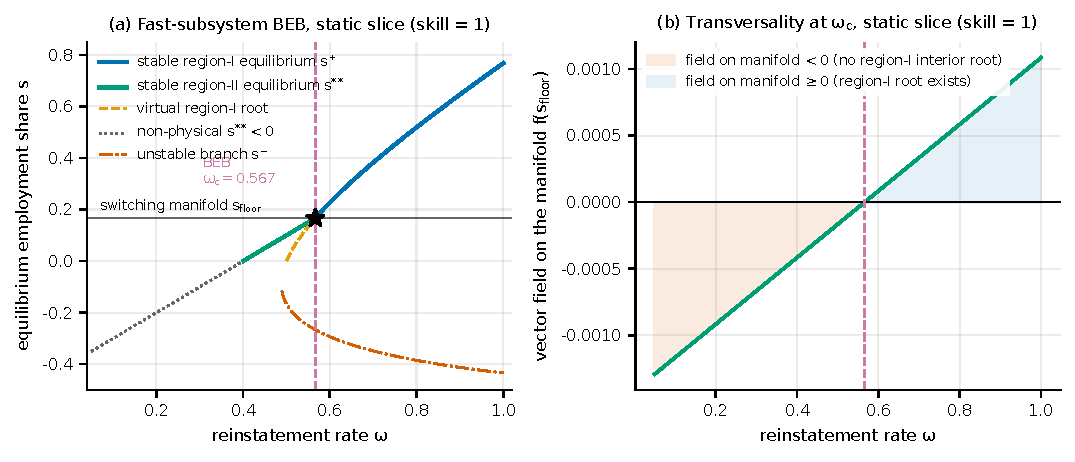
\includegraphics[width=0.98\textwidth]{fig_beb_static.pdf}
\caption{Boundary equilibrium bifurcation of the fast subsystem. Left: the physical equilibrium branch is absorbing at $s=0$ for $\omega<\kappa_I/q$, rises as a stable region-II (low-employment) equilibrium between $\kappa_I/q$ and $\omega_c$, and persists through the switching manifold $s_{\text{floor}}$ at $\omega_c=0.567$ into the stable region-I (high-employment) branch; virtual and non-physical roots are shown light. Right: the field on the manifold $f(s_{\text{floor}})$ crosses zero transversely at $\omega_c$.}
\label{fig:beb-static}
\end{figure}

\subsection{Endogenous reinstatement: policy as the bifurcation parameter}
In the baseline model $\omega$ is an exogenous constant, and its calibrated value $\omega=0.05$ lies far below $\omega_c$, so the bifurcation is real but unreachable and the collapse is inevitable under an unchanged policy rule. We now make $\omega$ endogenous. Public employment, workfare and retraining reattach workers to the production of new tasks, raising the share of new tasks that accrues to labor. Let $EP_t$ denote public-employment headcount, $TM_t$ workfare and transfer spending, and let the policy stock be
\begin{equation}
\Gamma_t=\gamma_{PE}\frac{EP_{t-1}}{L^S}
+\gamma_{TM}\frac{TM_{t-1}}{wL^S}
+\gamma_R\,\text{retrain}\cdot\text{skill}_{t-1},
\label{eq:endog-gamma}
\end{equation}
and set the reinstatement rate to
\begin{equation}
\boxed{\ \omega_t=1-(1-\omega_0)e^{-\Gamma_t}.\ }
\label{eq:endog-omega}
\end{equation}
This specification has the required properties. It is bounded, $\omega_t\in[\omega_0,1]$, monotone and smooth in each policy instrument, and saturating: with no policy it returns to the baseline $\omega_0$, and as the policy stock grows it approaches the pure social-welfare limit $\omega\to1$, in which new tasks accrue entirely to labor. Using the lagged stock in~\eqref{eq:endog-gamma} builds in the implementation delay.

\begin{proposition}[Policy crosses the bifurcation]
\label{prop:endog-cross}
There exists a finite policy stock $\Gamma_c=-\ln\!\bigl((1-\omega_c)/(1-\omega_0)\bigr)$ such that $\omega_t\ge\omega_c$ whenever $\Gamma_t\ge\Gamma_c$. Increasing any of $\gamma_{PE},\gamma_{TM},\gamma_R$ or the corresponding policy outlays lowers the time at which the threshold is reached and moves the system into the region with a stable high-employment equilibrium.
\end{proposition}
\begin{proof}
Solving~\eqref{eq:endog-omega} for $\Gamma_t$ at $\omega_t=\omega_c$ gives the stated $\Gamma_c$. The partial derivatives of $\omega_t$ with respect to each term in $\Gamma_t$ are positive, since $\partial\omega_t/\partial\Gamma_t=(1-\omega_0)e^{-\Gamma_t}>0$, and the equilibrium conclusion then follows from Theorem~\ref{thm:beb}.
\end{proof}

\subsection{Dynamic verification and the critical policy intensity}
The mechanism is verified on the full switching system. Figure~\ref{fig:beb-policy} contrasts three policy regimes. With no policy, $\omega_t$ stays below $\omega_c$, the employment share is absorbed toward zero and consumption breaks through its floor. Under the workfare corner with the baseline mapping, $\omega_t$ crosses $\omega_c$ and consumption is held at its floor even though the employment share continues to drift down under the inertia of the fast variable. Under the strong social floor, $\omega_t$ approaches $0.9$ and the employment share is retained above one half with consumption well above the floor.

\begin{figure}[htbp]
\centering
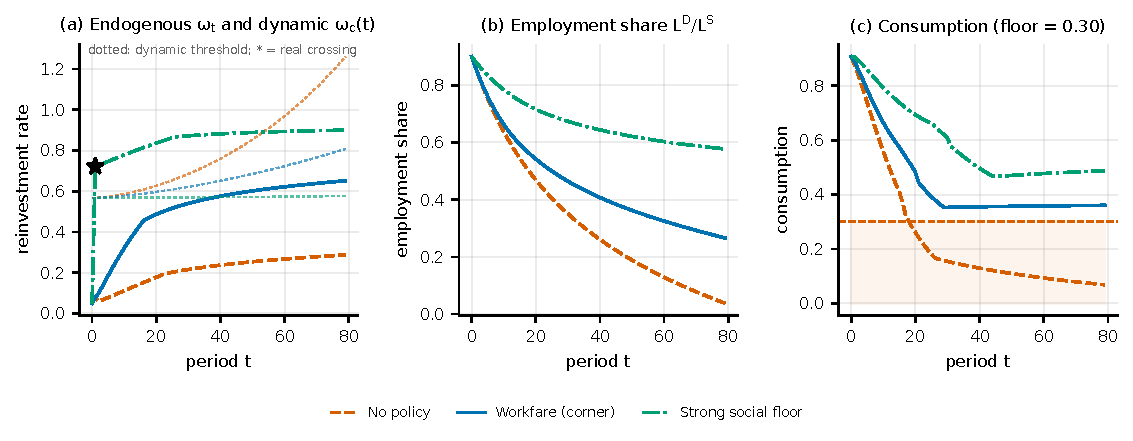
\includegraphics[width=1.0\textwidth]{fig_beb_policy.pdf}
\caption{Endogenous reinstatement and the resulting dynamic paths. (a) The endogenous rate $\omega_t$: the strong floor approaches $0.9$, the workfare corner crosses $\omega_c=0.567$, and the no-policy path stays below it. (b) Employment share and (c) consumption; the strong floor retains employment and consumption, the corner holds consumption at the $0.30$ floor, and the no-policy path collapses.}
\label{fig:beb-policy}
\end{figure}

A bisection on the public-employment intensity gives the sharp threshold for avoiding the crash, defined as $\min_t C_t\ge C_{\min}$:
\begin{equation}
p_E^{*}=0.4388,
\label{eq:beb-pestar}
\end{equation}
below which the economy crashes and above which consumption is defended. The long-horizon run ($T=200$) confirms the distinction: with no policy the employment share reaches zero at $t=91$ and $\min C=0.010$, whereas under the corner with transfers closed ($\phi^{\max}\to0$) the outcome is smooth with $\min C=0.302$, and under the strong floor the employment share ends at $0.506$ with $\min C=0.418$ and $\omega=0.914$.

\subsection{Slow--fast dynamics and the finite-rate lag}
The endogenous rate is a slow variable and the employment share is a fast variable,
\begin{equation}
\dot s=f(s,\omega),\qquad \dot\omega=\varepsilon\,g(\omega,\text{policy}),
\qquad 0<\varepsilon\ll1.
\label{eq:bif-slow}
\end{equation}
Away from the switching manifold the critical manifold $f=0$ is normally hyperbolic and the standard persistence theory applies~\citep{Fenichel1979}. Normal hyperbolicity is lost at the boundary equilibrium, where the fast variable cannot relax instantaneously; this is the piecewise-smooth analogue of the nonhyperbolic fold treated in geometric singular perturbation theory~\citep{KS2001,GH1983,Desroches2012}. It explains the lag visible in the simulations: after $\omega_t$ crosses $\omega_c$ the employment share keeps declining for several periods before arresting. Reducing the rate $\varepsilon$ at which the policy is pushed shrinks the lag, while raising the level of $\omega$ moves the equilibrium itself; the two are distinct instruments.

\subsection{Connection to the calibrated model}
\label{subsec:connection}
The high-employment region-I equilibrium corresponds structurally to the workfare corner policy $(\tau=0.15,p_E=0.45,\phi^{\max}=0.02)$ that avoids the crash in the social sweep, while the absorbing regime corresponds to the no-policy and pure-transfer collapses. The coefficients $\gamma_{PE},\gamma_{TM},\gamma_R$ and the baseline $\omega_0$ are structural parameters of the reduced subsystem, not externally estimated quantities, and the policy threshold $p_E^{*}=0.4388$ is a dimensionless output of the calibrated model under those baseline parameters---illustrative rather than an empirical estimate. A quantitative mapping from the analytic thresholds to the calibrated time path, including a microfoundation of the endogenous reinstatement law~\eqref{eq:endog-omega}, is left to future work.

\smallskip\noindent\textbf{Functional form of the saturation.}
Equation~\eqref{eq:endog-omega} is a modelling choice, so we re-solve the corner with two alternatives that share its endpoints ($\omega_0$ at $\Gamma=0$ and $\omega\to1$ as $\Gamma\to\infty$), its monotonicity and its smoothness: a rational form $\omega_t=\omega_0+(1-\omega_0)\Gamma_t/(1+\Gamma_t)$ and a linear-clipped form $\omega_t=\min\{1,\omega_0+\kappa\Gamma_t\}$, with $\kappa$ set so that the clipped and exponential forms agree at $\Gamma=1$. The critical stock moves with the form, $\Gamma_c=0.785$, $1.192$ and $0.860$ respectively, and so does the period of crossing: at the corner intensity the exponential and clipped forms cross $\omega_c$ at $t=38$ and $t=44$, whereas under the rational form the terminal rate is $0.542$ and $\omega_c$ is not reached inside the 80-period window. The buffer conclusion is unchanged by any of this: $\min_tC_t$ lies in $[0.305,0.306]$ and the total loss varies by $1.4\%$ across the three solutions. The reason differs. Under the exponential and clipped forms the floor is defended by the crossing itself, whereas under the rational form the employment share is absorbed more slowly and the window ends before the floor is tested, so its survival is a statement about the pace of the transition rather than about policy success. The crossing itself is form-dependent, but only through the product of form and elasticity: raising $\gamma_{PE}$ from $3.0$ to $4.8$ restores a crossing at $t=36$ under the rational form, so dynamics alone do not identify the two separately, and the reported $\Gamma_c$ and $p_E^*$ are statements about the baseline parameter pair rather than form-free constants.

% ============================================================================
\section{Calibration}
\label{sec:calibration}
% ============================================================================
\subsection{Parameter--data mapping}
Standardization $L^S=\barL=1$, $w=1$. In this section $\omega$ is held at its exogenous baseline, $\omega=0.05$, so every threshold reported below is the exogenous-reinstatement calibration. Section~\ref{sec:bifurcation} endogenizes $\omega$ and reports its own threshold, $p_E^{*}=0.4388$; the corner minima there differ in the third decimal from those below, and Section~\ref{subsec:connection} reconciles the two. Within the exogenous calibration used here, lowering the transfer ceiling to $\phi^{\max}=0.001$ at the fixed corner coordinates lowers $\min_tC_t$ from the headline $0.309$ at $\phi^{\max}=0.02$ to $0.306$, so the $0.003$ gap is the buffer carried by a two-percent transfer ceiling. What the model is anchored to, and where the anchoring stops, is the next matter.

\smallskip\noindent\textbf{What ``calibration'' means here.} Since the term can be read as claiming more than it delivers, we fix its sense before the table. Three entries are anchored to data: the consumption floor $q$ to the U.S. absolute poverty line, the transfer MPC $\mu_{TM}$ to the SNAP and CARES low-asset estimates, and the workfare wage ratio $w^P/w$ to workfare programmes. One group sits inside a literature range: the nominal-rigidity slopes $\gamma_p$ and $\lambda_w$ correspond to Calvo durations of roughly three quarters. The remaining entries are model-set by explicit convention. Among them $\kappa_I$ carries a distinct label, \emph{calibration target}: it is set so that the $T=80$ horizon reaches $s_t\to0$, which is the collapse the paper studies. Matching a parameter to a terminal condition is legitimate practice, but it means that statements of the form ``the transition completes within 80 periods'' restate the target rather than test it, and $\kappa_I$ is not an estimated displacement rate. The social channel ($\alpha_s,\varsigma^{th},J$) and the auxiliary accounting coefficients ($\theta,\zeta,\mu_d,\bar b,D_0,\delta_\sigma,g_{disp}$) are conventions as well. ``Calibrated'' therefore means three data-anchored magnitudes plus a two-parameter literature range, with everything else declared as setting; it does not mean that the parameter vector has been estimated, and no result below depends on reading it that way.

\begin{center}
\renewcommand{\arraystretch}{1.15}
\footnotesize
\begin{tabular}{@{}
>{\raggedright\arraybackslash}p{0.95in}
>{\raggedright\arraybackslash}p{1.35in}
>{\raggedright\arraybackslash}p{0.70in}
>{\raggedright\arraybackslash}p{2.80in}@{}}
\toprule
Param & Meaning & Baseline & Anchor / source \\
\midrule
$s_0=(N_0-I_0)/N_0$ & initial labor share & 0.90 & model initial state $I_0=0.20$, $N_0=2.00$ gives $s_0=0.90$; U.S.\ labor share 53.8\% is a benchmark only \emph{[model initial state; see note]} \\
$\kappa_I$ & automation displacement & 0.020 & transition (T$=$80) drives $s_t\to0$ \emph{[calibration target; set to hit $s_t\to0$ at $T{=}80$; not estimated]} \\
$g_A$ & automation frontier growth & 0.010 & long-run U.S.\ TFP $\approx1\%$/yr; the compute-cost decline is not used~\cite{HHSAI} \emph{[model-set; see note]} \\
$\eta$ & capital-tax growth inhibition & 0.40 & no direct anchor; a growth-inhibition coefficient, not a tax rate~\cite{DLL2014,OECD2026} \emph{[model-set; see note]} \\
$\gamma_p,\lambda_w$ & nominal rigidity & 0.15, 0.12 & Smets--Wouters Calvo $\zeta_p=\zeta_w=0.75$ (Nakamura--Steinsson; Bils--Klenow)~\cite{SW2007,NS2008,BK2004} \emph{[literature range]} \\
$\mu_{TM}$ & transfer MPC & 0.50 & USDA SNAP 0.30; CARES cumulative 0.66; low-asset 0.53; IMF 0.20; Miller 0.44--0.55~\cite{CM2019,CO2021,HLR2025} \emph{[verified against data]} \\
$q$ & consumption floor & 0.30 & U.S.\ absolute poverty line $\approx$ minimal food $\times3$ (ASPE/HHS) \emph{[verified against data]} \\
$\omega$ & reinstatement rate & 0.05 & A\&R: reinstatement weaker than displacement~\cite{AR2018} \emph{[model-set; direction grounded, magnitude not estimated]} \\
$w^P/w$ & workfare wage ratio & 0.85 & MGNREGA / World Bank workfare below market~\cite{Subbarao2013} \emph{[verified against data]} \\
\bottomrule
\end{tabular}
\end{center}

\noindent\footnotesize\textit{Note.} Three entries of the parameter table carry a ``see note'' flag. The initial share $s_0=0.90$ is computed from the task block itself, $s_0=(N_0-I_0)/N_0=(2.00-0.20)/2.00$, so it is an internal consistency requirement rather than a data target; the U.S.\ labor income share of 53.8\% (BLS, 2025Q3, incl.\ self-employment) serves only as a qualitative long-run benchmark, and the gap reflects that $s$ is a task/employment share rather than a wage-bill share and enters no equation. The frontier growth $g_A=0.01$ is set at the long-run U.S.\ TFP rate; the $-$30\%/yr hardware-cost decline and $+$40\%/yr efficiency gain reported by Stanford HAI 2025 / NVIDIA~\cite{HHSAI} refer to the cost of computing, not to $A_t$, and are deliberately not used as an anchor (sensitivity in Section~\ref{sec:calibration}). The inhibition coefficient $\eta=0.40$ scales the growth cost of the tax rate in $g_{eff}=g_G(1-\eta\tau)$ and is not an effective tax rate, so EATR levels (OECD 20.5\%, U.S.\ METR 18.3\%)~\cite{OECD2026} and tax-base elasticities ($-0.4$ total / $-0.7$ equipment)~\cite{DLL2014} serve as magnitudes only. Separately, the symbol $\sigma_t$ in this paper denotes the skill stock (Section~\ref{sec:technology}), not a capital--labor elasticity; the model has no CES production block. The broader elasticity range referenced in task-based calibrations (A\&R 2020 P\&P ICT $\eta\in(0.5,0.8)$; K\&N $>1$; mainstream $\approx1$) is background only and enters no equation~\cite{AR2020pandp,KN2014}.
\normalsize

\begin{center}
\renewcommand{\arraystretch}{1.15}
\footnotesize
\begin{tabular}{@{}
>{\raggedright\arraybackslash}p{0.95in}
>{\raggedright\arraybackslash}p{1.35in}
>{\raggedright\arraybackslash}p{0.70in}
>{\raggedright\arraybackslash}p{2.80in}@{}}
\toprule
Param & Meaning & Baseline & Anchor / source \\
\midrule
$\alpha_s$ & social-pressure coefficient & 0.60 & $\varsigma_t=\alpha_s\,U_t^{rem}/\barL$; relief share drives instability \emph{[model-set / calibration convention]} \\
$\varsigma^{th}$ & social-instability threshold & 0.50 & sustained $J=10$-period exceedance $\Rightarrow$ social collapse \emph{[model-set / calibration convention]} \\
$T$ & simulation horizon & 80 & transition window over which $s_t\to0$ is computed \emph{[model-set / calibration convention]} \\
$\delta_\sigma$ & skill depreciation & 0.015 & skill stock decay per period unemployed \emph{[model-set / calibration convention]} \\
$g_{disp}$ & automation output boost & 0.05 & $\delta_{disp}=(I_t-I_0)/N_0$ output dividend \emph{[model-set / calibration convention]} \\
$\theta$ & debt accumulation on gap & 0.10 & $D_t$ recursion coefficient \emph{[model-set / calibration convention]} \\
$\zeta$ & debt drag on consumption & 0.08 & $-\zeta\max\{0,b_t-\bar b\}$ \emph{[model-set / calibration convention]} \\
$\mu_d$ & monetary drag on consumption & 0.06 & $-\mu_d\max\{0,r_t^d\}$ \emph{[model-set / calibration convention]} \\
$\bar b$ & debt-drag threshold & 0.35 & real-debt trigger \emph{[model-set / calibration convention]} \\
$D_0$ & initial nominal debt (normalized) & 0.30 & initial balance sheet \emph{[model-set / calibration convention]} \\
\midrule
\multicolumn{4}{@{}p{6.3in}@{}}{\textit{Baseline policy levers.} $\tau=0.15$ (loss-minimizing corner on the reported grid), $p_E=0.45$ (workfare-dominant), $\phi^{\max}=0.02$ (the grid floor; transfers effectively closed under the baseline loss weights).} \\
\bottomrule
\end{tabular}
\end{center}

\smallskip\noindent\textbf{The transition-loss objective.}
The grid search ranks policies by a single scalar, and we therefore state that scalar explicitly instead of leaving it implicit in the simulation code. Writing $C^{fe}=w\barL$ for full-employment consumption, the objective for a policy path $(\tau,p_E,\phi^{\max})$ is
\begin{equation}
\mathcal{L}(\tau,p_E,\phi^{\max})
=\sum_{t=0}^{T}\Big[
\max(0,C^{fe}-C_t)
+\lambda\,TM_t
+\lambda_{PE}\,w^{P}EP_t+\nu\,EP_t^{2}
+\delta_\tau\,\tau^{2}\text{tax}_t
\Big],
\label{eq:loss}
\end{equation}
with $\lambda=0.5$, $\lambda_{PE}=0.6$, $\nu=0.5$ and $\delta_\tau=0.6$.
The four terms are all expressed in consumption units. The first is the consumption gap, the shortfall of realized consumption below what full employment at the prevailing wage would deliver. The second charges transfer outlays $TM_t$ at the leakage rate $\lambda$, reflecting that one yuan transferred raises consumption by $\mu_{TM}$ rather than by one. The third charges public-employment outlays at the workfare wage, $\lambda_{PE}w^{P}EP_t$, plus the congestion term $\nu EP_t^{2}$ that makes absorbing a large unemployed pool progressively more expensive. The fourth is the deadweight of the capital tax, quadratic in the rate so that it vanishes as $\tau\to0$ and produces the Laffer trade-off of Proposition~\ref{prop3b}.
Feasibility is a separate criterion and is not part of $\mathcal{L}$: a path is admissible if $C_t\ge C_{\min}=q\,w\barL$ for every $t\ge10$, the first ten periods being excluded to remove the initial-condition transient, and the statistic $\min_tC_t$ quoted throughout this section and in Figure~\ref{fig:baseline} refers to that window.
Proposition~\ref{prop3b} is the one-dimensional projection of \eqref{eq:loss}: with $p_E$ and $\phi^{\max}$ held fixed, the transfer and workfare charges collapse into its single $cost(\tau)$ term and the deadweight enters with the same quadratic form, so $W(\tau)$ and $\mathcal{L}$ rank policies identically along the $\tau$ axis.
The four weights are conventions rather than estimates: they set the relative price of a consumption shortfall, a fiscal outlay and a tax distortion, and no external data pin them down. What they do and do not control is reported below.

\paragraph{External ranges for the two policy instruments} Both instruments enter the closure mechanically, and two reduced-form ranges in the empirical literature can check those settings without becoming inputs. For workfare the relevant object is the employment multiplier: Lee, Ko and Kim~\cite{LeeKoKim2023} exploit public-sector relocations in South Korea as an exogenous source of public employment and estimate that one public-sector position raises private-sector employment by one, with the effect highly localized. Gechert~\cite{Gechert2015} reports a meta-regression over 104 studies in which public-spending multipliers are close to one and exceed those of tax cuts and transfers by 0.3--0.4. Our closure contains the direct positions and the demand they generate through the consumption block, but not a localized private-employment multiplier; the published one-for-one estimate therefore sits above what we model, and adding it would raise rather than lower the workfare ranking of Proposition~\ref{prop4}. For pure UBI the relevant object is the labor-supply response. Vivalt et al.~\cite{Vivalt2024} report, from the OpenResearch experiment that paid \$1{,}000 per month for three years to 1{,}000 low-income adults against 2{,}000 controls, a 2.0 percentage-point fall in labor-market participation and a 1.3--1.4 hour reduction in weekly hours. Our model has no hours margin, so a transfer leaves labor supply unchanged; that omission flatters pure UBI, since a smaller effective labor supply would shrink the tax base that has to carry the buffer. Both gaps therefore run in the direction that makes the ranking harder, not easier, to establish: the missing multiplier weakens workfare and the missing labor-supply response strengthens pure UBI. Filling either with the published range moves the comparison the same way. Neither range enters an equation, and this is the sense in which the policy claims are model-implied rather than universal.

\begin{figure}[htbp]
\centering
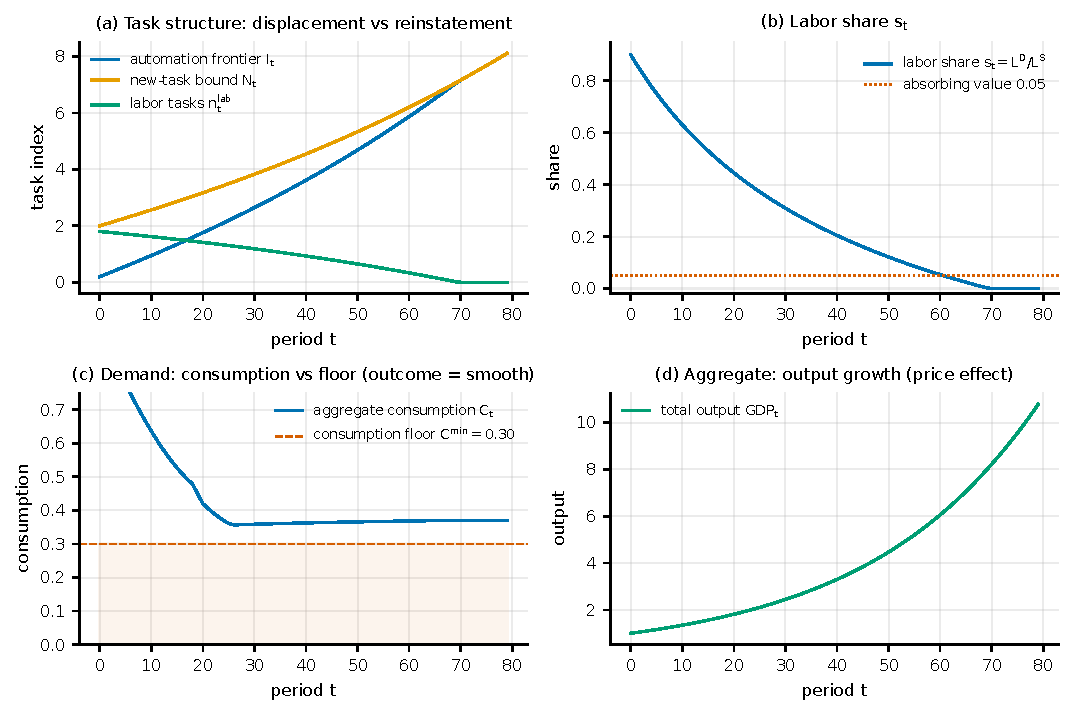
\includegraphics[width=0.98\textwidth]{fig_baseline.pdf}
\caption{Baseline smooth transition under the corner configuration $(\tau=0.15,p_E=0.45,\phi^{\max}=0.02)$ at the baseline frontier growth $g_A=0.010$. (a) The automation frontier $I_t$ and new-task bound $N_t$ diverge while labor tasks $n_t^{lab}$ vanish. (b) The labor share declines monotonically to its absorbing value. (c) Aggregate consumption stays above the floor $C^{min}=0.30$ (minimum $0.309$). (d) Total output keeps rising through the transition.}
\label{fig:baseline}
\end{figure}

\subsection{Robustness of the analytical results under the calibrated parameters}
Figure~\ref{fig:baseline} reports the baseline path under the corner configuration. Under the calibrated parameters ($\mu_{TM}=0.50$, $\eta=0.40$), transfers are costly relative to public-employment wages (one yuan of transfers yields $0.50$ of consumption, whereas a public-employment wage yields $1$), and the capital tax carries a Laffer supply-side cost. Running the full battery under the unified model engine yields the following calibrated outcomes:

\begin{center}
\small
\begin{tabular}{@{}
>{\raggedright\arraybackslash}p{1.55in}
>{\raggedright\arraybackslash}p{2.15in}
>{\raggedright\arraybackslash}p{2.45in}@{}}
\toprule
Result & Calibrated outcome & Conclusion \\
\midrule
Policy delay $d$ & corner ($\phi^{\max}{=}0.02$): $d{=}0$ and $d{=}12$ both smooth (0.309); standard ($\phi^{\max}{=}0.65$): $d{=}0$ crash (0.300), $d{=}12$ smooth (0.308) & delay immaterial at the corner; under the standard setting the delayed response is the smoother path \\
Isolation gain $\Delta$ vs $\omega$ & $0.02\to0.49$ & monotone, robust \\
Workfare vs UBI & $4/6$ not crashed vs $6/6$ crashed & workfare $>$ UBI at every $\omega$ \\
Minimum-loss point (grid) & $(0.15,0.45,0.02)$ & corner: workfare-dominant, close transfers, low tax \\
Feasible share, $p_E{=}0.45$ vs $0.30$ & $45.3\%$ vs $9.4\%$ & advantage retained \\
No-policy / pure-transfer & crash / all crash & buffering and financing necessary \\
\bottomrule
\end{tabular}
\\[2pt]
\footnotesize The feasible share is the fraction of the $8\times8$ $(\tau,\phi^{\max})$ cells at the stated $p_E$ that satisfy C1--C4, evaluated on the same wide grid as the count in Proposition~\ref{prop3a}: $29/64=45.3\%$ at $p_E=0.45$, $6/64=9.4\%$ at $p_E=0.30$, and $122/384=31.8\%$ over the grid as a whole. The workfare--UBI row counts six $\omega$ values at $(\tau=0.16,\phi^{\max}=0.65)$: workfare survives four of the six ($\omega=0.02$ and $0.05$ miss the floor at $0.293$ and $0.2999$), pure UBI crashes in all six, and workfare carries the lower total loss in all six.
\end{center}

\smallskip\noindent\textbf{The public-employment intensity is load-bearing.} The same six $\omega$ values at the corner $(0.15,0.02)$ survive at $p_E=0.45$ ($\min_tC_t=0.304$--$0.310$) but all collapse at $p_E=0.30$ ($\min_tC_t=0.197$--$0.218$, every path through the floor). The corner survives only above a public-employment share of roughly $0.45$, a feasibility bound rather than a tuning preference.



\textbf{Key calibrated narrative.} (i) The six analytical results P1--P6 are reproduced under the calibrated parameters within the reported grid; four are visible in this section: the reinstatement collapse drives $s_t\to0$; skill-retention value decays monotonically in $\omega$ (Figure~\ref{fig:skill-omega}); workfare ranks above pure UBI in the modeled crash channels; and the protective combination widens the surviving region. (ii) Under the baseline loss weights the minimum-loss point on the grid moves to a corner solution (workfare-dominant, transfers closed, minimal sufficient capital tax) driven by the MPC calibration. (iii) Within this calibrated model, no-policy and pure-transfer regimes are infeasible under the unified engine (financing-constraint collapse), reinforcing the paper's model-implied message: \emph{a smooth transition requires a policy buffer and that the buffer be financed}. Figure~\ref{fig:policy-compare} contrasts the three regimes on the consumption margin.

\smallskip\noindent\textbf{Sensitivity to $g_A$ and $\eta$.} Two calibration entries admit no verifiable external anchor, the automation-frontier growth $g_A$ and the capital-tax growth inhibition $\eta$, so we sweep both and report the outcome instead of asserting that the baseline values are innocuous. Varying $g_A$ over $\{0.010,0.05,0.10,0.20,0.30\}$ at the corner gives minimum consumption $0.309,0.283,0.228,0.166,0.150$ and outcome smooth, crash, crash, crash, crash. The smooth corner therefore survives only at $g_A=0.010$: at $g_A=0.05$, one sixth of the $-$30\%/yr hardware-cost decline often quoted for computing, the floor is already breached ($\min_tC_t=0.283<0.30$), and at $g_A\ge0.20$ the transition crashes hard with an unbounded loss. This is the sharpest sensitivity in the calibration, and the smooth conclusion should be read as conditional on a conservative long-run-TFP frontier growth rate rather than on a hardware-cost rate. By contrast $\eta$ is nearly inert over the admissible tax range: sweeping $\eta$ from $0.20$ to $0.80$ leaves every corner outcome smooth at $\min_tC_t=0.309$ and moves the total loss by less than $0.1\%$, so the imprecision of $\eta$ affects no conclusion, while also implying that no sharp Laffer effect can be claimed at $\tau=0.15$. Both sweeps are reproducible from the replication script with the corner configuration.

\begin{figure}[htbp]
\centering
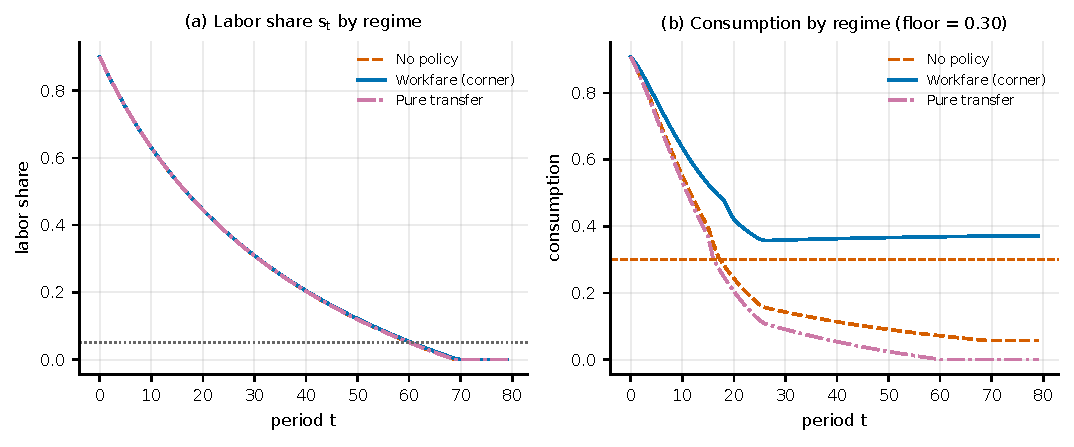
\includegraphics[width=0.98\textwidth]{fig_policy_compare.pdf}
\caption{Policy-regime comparison. (a) The labor share $s_t$ follows the same task-driven decline under all three regimes. (b) The workfare corner holds aggregate consumption above the floor, whereas the no-policy and pure-transfer regimes fall below it and become infeasible; the consumption buffer, not the market employment count, is what distinguishes the regimes.}
\label{fig:policy-compare}
\end{figure}

\smallskip\noindent\textbf{Grid minima and identification.} Figure~\ref{fig:loss-surface} visualizes the loss surface. Three minima are reported. A scan that fixed $\phi^{\max}=0.15$ returns $(0.18,0.40,0.15)$ with loss $67.20$; the wide grid, which extends $\phi^{\max}$ down to $0.02$, returns the corner $(0.15,0.45,0.02)$ with loss $66.86$; and a denser grid that extends $\phi^{\max}$ to $0.001$ returns $(0.13,0.44,0.001)$ with loss $66.70$, taken up below. The three are ordered monotonically in the ceiling---the lower the cap on transfers, the lower the minimized loss---with a total spread below $0.8\%$. The loss surface is locally flat, so the exact coordinates are grid-dependent rather than sharply identified. We report the wide-grid corner as the headline because it retains a visible buffer.

A refinement test addresses the boundary directly. Re-solving on a denser grid---capital-tax step $0.01$, workfare step $0.02$, and $\phi^{\max}$ extended down to $0.001$---moves the minimizer to $(0.13,0.44,0.001)$ with loss $66.70$, against $66.86$ on the wide grid, a relative difference of $0.24\%$. The transfer ceiling is monotone in the same direction: holding $(\tau,p_E)=(0.15,0.45)$, lowering $\phi^{\max}$ from $0.10$ to $0.001$ lowers the loss from $66.91$ to $66.85$ and $\min_tC_t$ from $0.323$ to $0.306$. Closing transfers is therefore a preference of the objective rather than a grid-resolution artifact, but two caveats remain. The exact corner coordinates are not identified, and the denser solution carries almost no buffer: $\min_tC_t=0.3004$ against a floor of $0.300$, so it clears by four ten-thousandths. The refined solution is reported here to show what the objective does once the grid stops being the binding constraint.

\begin{figure}[htbp]
\centering
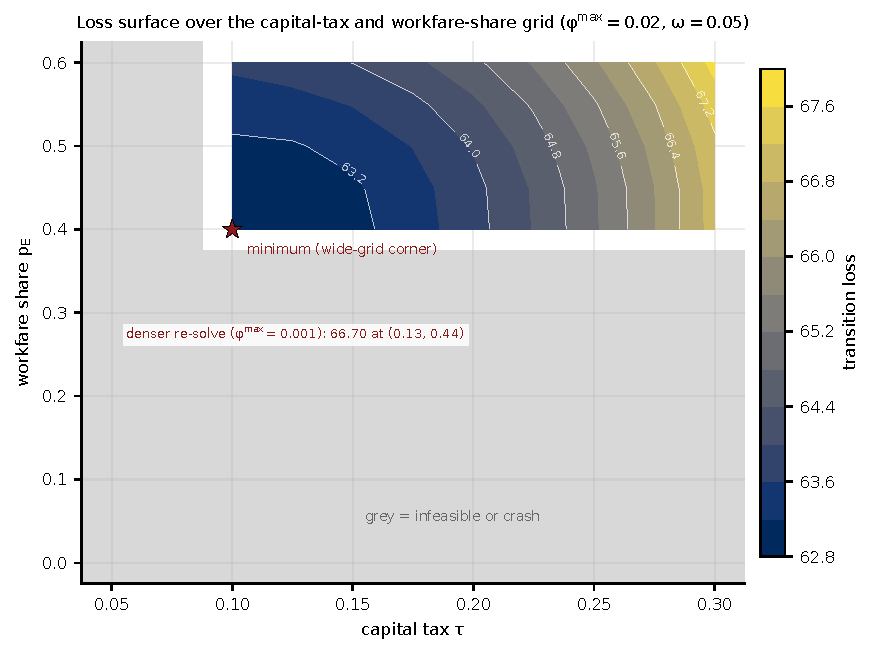
\includegraphics[width=0.92\textwidth]{fig_loss_surface.pdf}
\caption{Transition loss over the capital-tax and workfare-share grid at $\phi^{\max}=0.02$, $\omega=0.05$. The grey region is infeasible (crash); the smooth region is confined to high workfare shares, and under the baseline loss weights the loss-minimizing point on this grid sits at its corner (solid star). The smooth surface is locally flat, so the minimizer's exact coordinates are grid-dependent rather than identified. A denser re-solve that extends $\phi^{\max}$ to $0.001$ moves the minimizer to $(0.13,0.44)$ with a loss of $66.70$ (stated in the panel); that location is not a point on the $\phi^{\max}=0.02$ surface drawn here, which is why it is reported in words rather than marked.}
\label{fig:loss-surface}
\end{figure}

\smallskip\noindent\textbf{Sensitivity to the loss weights.}
The weights in \eqref{eq:loss} are conventions, so we report what they do and do not control rather than asserting that they are innocuous. Feasibility is weight-independent by construction: re-ranking all $384$ grid points under six weight configurations leaves the admissible set at $122$ points in every case, so whether a path is smooth or crashes does not depend on $\lambda$, $\lambda_{PE}$, $\nu$ or $\delta_\tau$, and the feasible shares reported above are unaffected. The ranking among admissible paths does depend on them. The corner $(0.15,0.45,0.02)$ is selected in four of the six configurations, including a doubling and a halving of the deadweight weight ($\delta_\tau=1.2$ and $\delta_\tau=0.2$), which change the minimized loss by less than $1\%$. The remaining two configurations move the minimizer: halving the cost weights relative to the gap gives $(0.25,0.55,0.65)$ with $\min_tC_t=0.429$, and doubling them gives $(0.15,0.40,0.15)$ with $\min_tC_t=0.307$. In every configuration public employment remains the dominant instrument, with $p_E\in[0.40,0.55]$, whereas the transfer ceiling ranges from $0.02$ to $0.65$. Workfare dominance is thus a property of the model, while the statement that transfers are closed at the optimum is a property of the baseline weights together with the lower grid bound, and is reported as such.

\smallskip\noindent\textbf{Stochastic robustness.} The analytical results are deterministic, and a deterministic path should not be presented as if it stood in for a stochastic one. We therefore shock the frontier growth itself, the parameter on which the smooth conclusion most depends. The growth rate becomes $g_{A,t}=0.010+\varepsilon_t$ with an AR(1) deviation ($\rho=0.5$, Gaussian innovations of standard deviation $\sigma$ (the shock scale, distinct from the skill index $\sigma_t$)), the engine is otherwise unchanged, and each configuration is run $200$ times; a path is recorded as a crash when it triggers the economic or social crash test before the horizon ends. Table~\ref{tab:shock} reports the results.

\begin{table}[h]
\centering\small
\caption{Monte Carlo crash counts under frontier-growth shocks ($200$ replications; AR(1), $\rho=0.5$). Buffer is $\min_tC_t-0.300$; the last column reports the fifth percentile of $\min_tC_t$ at $\sigma=0.03$.}\label{tab:shock}
\begin{tabular}{@{}lccccc@{}}
\toprule
Configuration & buffer & $\sigma{=}0.01$ & $\sigma{=}0.02$ & $\sigma{=}0.03$ & $\min_tC_t$, 5\% \\
\midrule
Headline $(0.15,0.45,0.02)$ & $0.009$ & $0/200$ & $1/200$ & $6/200$ & $0.3046$ \\
Denser $(0.13,0.44,0.001)$ & $0.0004$ & $78/200$ & $126/200$ & $143/200$ & $0.2738$ \\
\bottomrule
\end{tabular}
\end{table}

Two things follow. First, the headline configuration survives shocks of the size considered: with $\sigma=0.01$---a frontier-growth innovation as large as the baseline rate itself---none of the $200$ paths crashes, and even at $\sigma=0.03$ only $6$ do; a further $26$ at that scale are paths that fail to drive the labor share to its absorbing value within $T$ because the shock raises the frontier, which we count as neither survival nor crash. Second, what buys this is the margin, not the policy design as such. The denser minimum-loss configuration, which clears the floor by $0.0004$, loses $39\%$ of its paths at $\sigma=0.01$ and $72\%$ at $\sigma=0.03$, and its fifth-percentile minimum consumption falls to $0.274$. Minimizing the loss therefore pushes the design toward the floor, and the buffer that makes the headline robust is a property of the reported corner rather than of the objective's minimizer. This is the quantitative counterpart of the qualitative statement above: the buffer buys time, and its thickness determines how much. Demand-side, monetary and policy-implementation shocks are not modelled, and a fully stochastic version of the model remains for future work (Section~\ref{sec:conclusion}).

\smallskip\noindent\textbf{Two configurations, not one.} The smooth headline depends on the corner configuration. At the baseline $\omega=0.05$, the wide-grid corner $(0.15,0.45,\phi^{\max}=0.02)$ runs smooth with $\min C=0.309>C^{min}=0.30$. Under the standard setting $(\tau=0.16,p_E=0.45,\phi^{\max}=0.65)$ used in the social-channel comparison of Table~\ref{tab:socbase}, the standard-setting points $(0.16,0.30,0.65)$ and $(0.16,0.45,0.65)$ instead crash with $\min C=0.276$ and $0.2999$. Smoothness therefore obtains only once $\phi^{\max}$ is driven near zero; the paper does not claim that workfare survives at the baseline under the looser standard setting.

\begin{figure}[htbp]
\centering
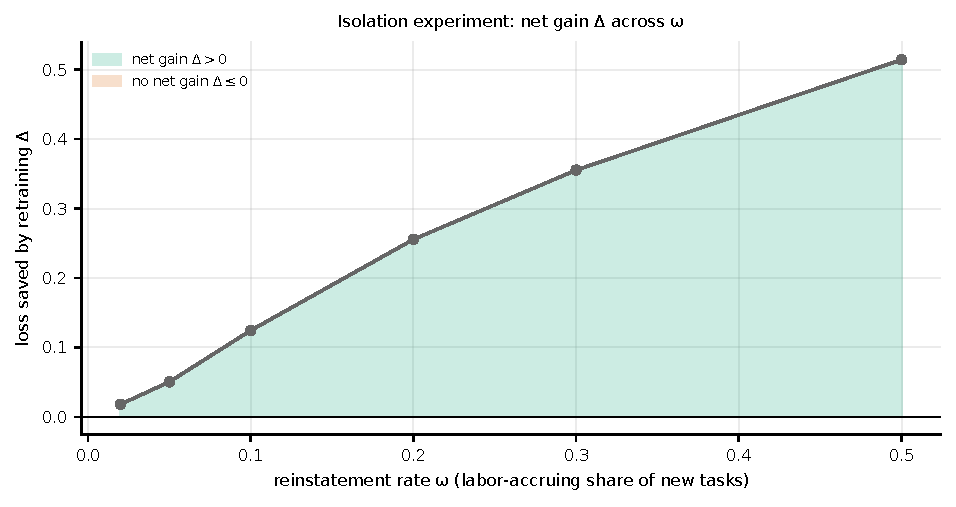
\includegraphics[width=0.84\textwidth]{fig_skill_omega.pdf}
\caption{Isolation experiment: the loss saved by retraining $\Delta$ rises monotonically with the reinstatement rate $\omega$, the share of new tasks accruing to labor. As $\omega\to0$ (AGI takes over new-task creation and reinstatement fails), the value of retraining vanishes, confirming that skill retention pays off only while labor can still capture new tasks.}
\label{fig:skill-omega}
\end{figure}

\smallskip\noindent\textbf{Social-threshold sensitivity sweep.} A dedicated social-channel sweep uses the model engine and varies one social-channel parameter at a time: $\varsigma^{th}$ over $0.20$--$0.70$, $\alpha_s$ over $0.30$--$1.20$, and $J$ over $3$--$30$, plus a two-dimensional $\varsigma^{th}\times\alpha_s$ grid, under the calibrated parameters ($\eta=0.40,\mu_{TM}=0.50$). Three policies are compared: the recommended corner $(\tau=0.15,p_E=0.45,\phi^{\max}=0.02)$, the standard setting $(\tau=0.16,p_E=0.45,\phi^{\max}=0.65)$, and pure UBI $(p_E=0)$ as the extreme social-channel case. Table~\ref{tab:socbase} reports baseline outcomes; Table~\ref{tab:socbound} reports the stability/crash boundaries.

\begin{table}[h]
\centering\small
\caption{Baseline social-channel outcomes ($\varsigma^{th}=0.50,\alpha_s=0.60,J=10$, $g_A=0.010$). Values within $10^{-3}$ of the floor are given to four decimals.}\label{tab:socbase}
\begin{tabular}{@{}lccccc@{}}
\toprule
Policy & outcome & crash type & $\min C$ & peak stress & social crash \\
\midrule
Corner $(0.15,0.45,0.02)$ & smooth & none & 0.309 & 0.330 & no \\
Standard $(0.16,0.45,0.65)$ & crash & econ & 0.2999 & 0.330 & no \\
Pure UBI $(0.16,0,0.65)$ & crash & both & 0.210 & 0.600 & yes \\
\bottomrule
\end{tabular}
\end{table}

\begin{table}[h]
\centering\small
\caption{Social-crash boundaries under one-at-a-time sweeps.}\label{tab:socbound}
\begin{tabular}{@{}lccc@{}}
\toprule
Swept parameter (baseline) & Corner & Standard & Pure UBI \\
\midrule
critical $\varsigma^{th}$ (base 0.50) & $0.33$ & $0.33$ & $0.60$ \\
critical $\alpha_s$ (base 0.60) & $0.91$ & $0.91$ & $0.50$ \\
critical $J$ (base 10) & never triggers & never triggers & all $J\in[3,30]$ \\
\bottomrule
\end{tabular}
\\[2pt]
\footnotesize Values below/above the boundary trigger the social crash; for $\varsigma^{th}$ a lower value triggers, for $\alpha_s$ a higher value triggers.
\end{table}

\noindent The two-dimensional grid for the corner (S = social crash, . = no social crash) traces the same boundary:
\begin{center}\small
\begin{tabular}{@{}l|ccccc@{}}
\toprule
$\varsigma^{th}\backslash\alpha_s$ & 0.45 & 0.60 & 0.75 & 0.90 & 1.20 \\
\midrule
0.25 & . & S & S & S & S \\
0.30 & . & S & S & S & S \\
0.33 & . & . & S & S & S \\
0.40 & . & . & S & S & S \\
0.50 & . & . & . & . & S \\
\bottomrule
\end{tabular}
\end{center}

\noindent\textbf{Mechanism.} At $p_E=0.45$, public employment absorbs 45\% of the unemployed and only 55\% remain on pure relief, so $\varsigma_t=\alpha_s(1-p_E)u_t=0.55\,\alpha_s u_t$, peaking at $0.55\,\alpha_s\,u^{max}=0.330$ at the baseline $\alpha_s=0.60$ with $u^{max}=1$, which is 34\% below the $0.50$ cutoff. The analytic boundaries are therefore exact: $\varsigma^{th}_{crit}=0.33$ and $\alpha_s^{crit}=0.50/0.55=0.909$. In the run that tightens the cutoff toward the boundary, the first sustained exceedance occurs late in the transition (periods 24--55 under the $\varsigma^{th}$ scan), consistent with stress building only as unemployment approaches its peak. Under pure UBI, $100\%$ of the unemployed stay on relief and $\varsigma_t$ peaks at $\alpha_s=0.60>0.50$, triggering the social channel at the baseline.

\noindent\textbf{Conditional conclusion.} The workfare-over-UBI ranking does \emph{not} flip within the scanned range; the sweep strengthens it. To make the recommended corner socially crash, $\varsigma^{th}$ would have to fall from $0.50$ to below $0.33$ (a 34\% reduction) or $\alpha_s$ rise from $0.60$ to above $0.91$ (a 52\% increase), while pure UBI already socially crashes at the baseline. The persistence count $J$ is immaterial to the corner because stress never exceeds the cutoff at baseline. The ranking remains conditional on the reduced-form cutoffs, whose external empirical anchoring we examine separately (Section~\ref{sec:social-anchor}); it is backed by quantified robustness margins rather than a qualitative caveat.

\subsection{External empirical anchoring of the social-instability parameters}
\label{sec:social-anchor}

The social-instability channel contains three reduced-form parameters: the social-crash cutoff $\varsigma^{th}$ (baseline $0.50$), the stress coefficient $\alpha_s$ (baseline $0.60$), and the sustained-exceedance window $J$ (baseline $10$ periods, one model period being one year). We search the empirical literature for mappable evidence for each parameter, distinguish direct anchors from indirect (directional) evidence, and state the mapping assumptions explicitly. Table~\ref{tab:anchor-status} summarizes the anchoring status.

\begin{table}[h]
\centering\small
\caption{External empirical anchoring status of the three social-instability parameters.}\label{tab:anchor-status}
\begin{tabular}{@{}
>{\raggedright\arraybackslash}p{0.8in}
>{\raggedright\arraybackslash}p{0.7in}
>{\raggedright\arraybackslash}p{1.7in}
>{\raggedright\arraybackslash}p{2.6in}@{}}
\toprule
Parameter & Baseline & Anchoring status & Nature of evidence \\
\midrule
$\varsigma^{th}$ & 0.50 & no direct external anchor & directional/continuous probability only; no normalized cutoff \\
$\alpha_s$ & 0.60 & partially anchored & reverse-engineered range $0.5$--$2.5$; 0.60 at the lower end \\
$J$ & 10 & partially anchored & mean/upper-tail scale (crisis 8--10 yrs; civil-war mean 11.1 yrs) \\
\bottomrule
\end{tabular}
\end{table}

\paragraph{The cutoff $\varsigma^{th}=0.50$: no direct external anchor} No study provides a population-dependency threshold that maps onto a $0.50$ cutoff of the $[0,1]$ normalized stress variable. The authoritative literature consistently reports continuous probability or dose--response relationships rather than structural thresholds replicable across samples. Using rainfall as an instrument across 41 African countries over 1981--1999, Miguel, Satyanath and Sergenti~\cite{MSS2004} identify that a five-percentage-point drop in real GDP growth raises the probability of conflict in the following year (at least 25 battle deaths) by about 12 percentage points, a relative increase of roughly 50\%. Ponticelli and Voth~\cite{PV2020}, across 25 European countries over 1919--2008, find that a one-standard-deviation spending cut (about 2.8 percentage points of GDP) adds roughly 0.4 unrest events per year, with the event count nearly doubling as cuts widen from 1\% to 10\% of GDP; only a descriptive soft cutoff around a 2\%-of-GDP cut appears, not an identified structural threshold. Using natural disasters as instruments, Bellemare~\cite{Bellemare2015} identifies that a one-unit rise in the global food price index adds about 0.99 food-related unrest reports per month, while price volatility has no significant effect. Earlier work by Collier and Hoeffler~\cite{CH2004}, Fearon and Laitin~\cite{FL2003}, and Alesina and Perotti~\cite{AP1996} likewise reports continuous marginal effects. The only explicit numerical cutoff, due to Lagi, Bertrand and Bar-Yam (2011, arXiv:1108.2455, not peer reviewed), clusters protests when the FAO food price index exceeds 210; but that cutoff is a price-index level rather than a population dependency ratio, and mapping it onto $\varsigma^{th}=0.50$ would require an over-long chain of normalization assumptions, so we do not adopt it as a direct anchor.

\paragraph{The stress coefficient $\alpha_s=0.60$: partially anchored, with an identifiable range} The sign with which unemployment or relief dependence raises property crime and social unrest is robust across U.S., European and cross-country panels, ruling out $\alpha_s\leq 0$. The literature reports crime semi-elasticities to unemployment of roughly $+1.3\%$ to $+4\%$ per percentage point of unemployment, concentrated in property crime with weak effects on violent crime. Raphael and Winter-Ebmer~\cite{RWE2001} find that a one-percentage-point fall in unemployment lowers property crime by about 1.6\%--2.4\%; Lin~\cite{Lin2008} identifies a 1.8\% OLS and 4.0\% 2SLS rise in property crime per extra percentage point of unemployment; Gould, Weinberg and Mustard~\cite{GWM2002} find that the 23.3\% decline in low-skill male wages over 1979--1993 accounts for 43\% of the rise in property crime; Buonanno, Drago and Galbiati~\cite{BDG2014}, across about 20 developed countries over 1970--2010, identify a roughly 1.3\% rise in total crime and 1.7\% rise in homicides per extra percentage point of unemployment; and Foug\`ere, Kramarz and Pouget~\cite{FKP2009} identify a significant positive effect of youth unemployment on property crime in France; see also the surveys by Freeman~\cite{Freeman1999} and Draca and Machin~\cite{DM2015}. Mapping these semi-elasticities $\beta_{crime}\approx\partial\log C/\partial u$ onto $\alpha_s=\partial\,\text{stress}/\partial r$ requires three layers of assumptions: (A) the normalized range linking the stress index to disorder indicators, setting $\text{stress}=1$ to correspond to a 3--10-fold amplification of crime over baseline (mapping slopes of about 0.43--0.91); (B) the conversion factor $k=r/u$ between the relief share $r$ and unemployment $u$ (about $0.4$); and (C) a local linearization treating the semi-elasticity as approximately constant over the working range. Under transparent versions of these assumptions, $\alpha_s\approx f'\beta_{crime}(1/k)$ reverse-engineers a defensible range of about $0.5$--$2.5$. The baseline $0.60$ sits at the lower end of this range: neither rejected nor specifically supported by the literature, it is a reasonable but conservative calibration rather than an empirically identified value.

\paragraph{The sustained-exceedance window $J=10$: partially anchored at mean/upper-tail scale} No study directly estimates the window of consecutive stress exceedance that triggers a crash. Annual-scale evidence brackets ten years along two independent lines. First, after systemic banking crises, per-capita GDP returns to its pre-crisis peak in about eight years on average (median 6.5 years), with 45\% of episodes experiencing a second dip~\cite{RR2014}; Cerra and Saxena~\cite{CS2008} find highly persistent, near-permanent output losses after banking crises, with later estimates placing the average post-crisis GDP loss at about ten years. Second, civil wars last 11.1 years on average (median 7.1 years)~\cite{Fearon2004}, and the hazard estimates of Collier, Hoeffler and S\"oderbom~\cite{CHS2004} average just over seven years, with wars begun in the 1980s lasting 105 months (about 8.75 years). On the other side, protest waves and crime shocks persist only months to 2--5 years, markedly shorter than ten years. $J=10$ is therefore a defensible mean/upper-tail anchor aligned with chronic post-crisis slumps and average civil wars, but it lies above the median durations and should be read as such rather than as a median anchor.

\paragraph{Parameter decision and empirical-range robustness} Because none of the three parameters has a precise, directly identified empirical replacement, and the baseline values all lie within defensible empirical ranges, we do not adjust the baseline: assigning a value to $\varsigma^{th}$ would lack mappable threshold evidence; $\alpha_s=0.60$ lies inside the reverse-engineered range $0.5$--$2.5$; and $J=10$ is a supported mean/upper-tail value. A dedicated empirical-range sweep extends the $\alpha_s$ scan across the full $0.5$--$2.5$ range alongside a directional $\varsigma^{th}$ scan. The analytic boundaries are $\alpha_s^{crit}=0.50/((1-0.45)u^{max})=0.909$ (with $u^{max}=1$) and $\varsigma^{th}_{crit}=0.33$, and the numerical sweep locates the first social crash at $\alpha_s=0.91$ (smooth at $0.90$) and between $\varsigma^{th}=0.30$ and $0.33$ (smooth at $0.33$); $\min C$ stays $0.309$ throughout because the social channel does not feed back into the economic paths. The first sustained exceedance occurs late in the transition (periods 24--70 in the $\alpha_s$ sweep). The baseline conclusion does not flip: the corner stays smooth at the baseline and across the lower empirical range, turning to a social crash only when $\alpha_s$ rises above $0.91$ or $\varsigma^{th}$ falls below $0.33$; the sweep thereby bounds the channel's fragility to high-end parameter values.

% ============================================================================
\section{Contribution to the Literature}
\label{sec:literature}
% ============================================================================
The existing AGI macroeconomics literature addresses the transition along three separate axes. Restrepo (2025) and Korinek--Suh (2024) characterize the \emph{supply-side} conditions under which automation collapses wages; Fornaro--Wolf (2026) trace the \emph{demand-side} channel from income shifts to the natural rate; and the fiscal-instrument literature treats taxes and transfers as optimal-schedule objects. What none of them does is join the axes, so that the size and the financing of the buffer and the existence of the high-employment branch are decided together rather than separately. This paper proposes a two-layer task model that:

\begin{enumerate}
\item \textbf{Endogenizes the reinstatement collapse} (driven by AGI participation $\kappa_N^{AI}$ and the reinstatement rate $\omega$), proving the labor share vanishes monotonically (Theorem~\ref{thm1}), and shows skill-retention value decays with $\omega$, with no value as $\omega\to0$.
\item \textbf{Upgrades Fornaro--Wolf's demand shortfall into a decidable deflationary spiral} (Theorem~\ref{thm2}), cascading the collapse source (Theorem~\ref{thm1}) into crash dynamics.
\item \textbf{Characterizes the fiscal closure}: a Laffer interior tax $\tau^*$ (Proposition~\ref{prop3b}) and within-budget superiority of public employment over transfers (Proposition~\ref{prop4}).
\item \textbf{Introduces a social-instability channel independent of economic deflation}, proving workfare dominates pure UBI for social-instability risk (Proposition~\ref{prop5}), complementing the qualitative Tcherneva/Ravallion debate and the basic-income-versus-job-guarantee comparison of Mitchell and Watts~\cite{Tcherneva,Ravallion,MitchellWatts2004}.
\item \textbf{Establishes a robustness ceiling for the buffer family} (Proposition~\ref{prop6}): strong shocks require supply-side structural measures, a result absent from the literature.
\item \textbf{Closes the open question on the reinstatement rate with an analytic bifurcation theory}. Acemoglu--Restrepo treat $\kappa_N$ (in their notation) as an exogenous constant and leave its determinants open; we derive the fast subsystem directly from the model and show that the high-employment branch is lost through a boundary equilibrium bifurcation at the piecewise-smooth switching manifold. This yields a closed-form critical reinstatement rate, an endogenous policy rule that moves the system across the bifurcation, and a finite-rate lag between the slow policy and fast employment variables (Section~\ref{sec:bifurcation}). The reduction is a local statement whose parameters are dimensionless and illustrative rather than estimated, so the claim is structural rather than quantitative.
\end{enumerate}

Calibration anchors three magnitudes to data (the consumption floor, the transfer MPC and the workfare wage ratio); the initial labor share $s_0=0.90$ follows from the model's own task block, the U.S.\ labor share of 53.8\% is a qualitative benchmark rather than a target, and the elasticity range and the $-$30\%/yr compute-cost decline are background and enter no equation (Section~\ref{sec:calibration}). The grid search returns a ``workfare-dominant + capital-tax-financed'' corner whose coordinates are grid-dependent rather than uniquely identified, providing an analyzable and quantitative basis for a smooth AGI transition.

Related empirical work grounds the task and labor-share foundations. The skill-content framework originates with Autor, Levy and Murnane~\cite{ALM2003}; exposure to robots is estimated to reduce local employment and wages~\cite{AR2020}; and the declining labor share is linked to the reallocation of value toward superstar firms~\cite{ADKPV2020}. Broader policy-oriented analyses emphasize the distributional harms of AI deployed along its current trajectory~\cite{Acemoglu2021} and the need for development strategies that share the gains from artificial intelligence more widely~\cite{KS2021}.

Several recent papers address adjacent mechanisms, and in each case the difference lies along a specific axis. Atolia, Holland and Kreamer~\cite{Atolia2024} solve for the majority-voting optimal capital tax and basic income after an episode of automation, characterizing long-run outcomes and transitional welfare. Their policy is an optimal tax--transfer schedule; ours treats the two instruments as parameters of a bifurcation unfolding and asks when the high-employment branch ceases to exist. Kleven and Zidar~\cite{KlevenZidar2026} characterize optimal labor and capital income taxation in a task-based automation model calibrated to the U.S. wage distribution, and find a sizable optimal capital tax that is, in their benchmark, unaffected by automation. Our capital tax is not an optimal-tax object: it is the financing instrument of the buffer, and what matters for us is the tax base, which shrinks as $s_t\to0$, so the constraint we identify is fiscal feasibility rather than tax optimality. Ray and Mookherjee~\cite{RayMookherjee2022} derive the long-run labor share in a growth framework where automation moves the share along a smooth path; we study the case in which the reinstatement engine itself collapses, so the share is lost through a branch disappearance rather than a continuous decline. Nakamura and Zeira~\cite{NakamuraZeira2024} analyze transitional unemployment dynamics and identify conditions under which assistance arrives in time; their object is the unemployment stock, ours is the existence of an equilibrium branch. Bond and Kremens~\cite{BondKremens2024} characterize income and inequality under asymptotically full automation, a steady-state distribution question, whereas our constraint is fiscal feasibility along the transition. Jacobs~\cite{Jacobs2023} studies capitalist--worker wealth distribution in a task-based model without a policy-instrument bifurcation, and Stiefenhofer~\cite{Stiefenhofer2025} analyzes AGI substitution inside a CES production structure, where substitution is continuous across factors; our production structure is task-based, so substitution occurs at task boundaries and the resulting instability is discrete.

% ============================================================================
\section{Conclusion}
\label{sec:conclusion}
% ============================================================================
This paper has built a task-based macroeconomic model of the AGI labor transition that integrates, in one numerically solvable system, the supply side (endogenous reinstatement collapse), the demand side (debt-deflation at the zero lower bound), the fiscal side (capital-tax financing of workfare and transfers), and a social-instability channel. Its results fall into three groups. On the \emph{mechanism}, reinstatement collapse drives the labor share monotonically to zero with no self-correction, and the demand block turns that collapse into a decidable deflationary spiral rather than a shortfall (Theorems~\ref{thm1} and~\ref{thm2}). On the \emph{fiscal design}, a smooth-transition region exists with a Laffer interior capital tax (Propositions~\ref{prop3a}--\ref{prop3b}); public employment dominates transfers within the budget and protects better than pure UBI against social-instability risk (Propositions~\ref{prop4}--\ref{prop5}); and the buffer family has a robustness ceiling beyond which only supply-side measures help (Proposition~\ref{prop6}). On the \emph{method}, Section~\ref{sec:bifurcation} identifies the collapse as a boundary equilibrium bifurcation of the piecewise-smooth fast subsystem, giving a closed-form critical reinstatement rate, making that rate endogenous to public employment, workfare and retraining so that policy can move the system across the bifurcation, and characterizing the finite-rate lag between slow policy and fast employment.

The policy implications follow, within this calibrated model, rather than as universal claims. A smooth transition is not automatic: it requires an explicit policy buffer, and that buffer must be financed. Under the calibrated parameters and at the baseline frontier growth $g_A=0.010$, the loss-minimizing design on the reported grid is workfare-dominant (a public-employment floor that converts relief recipients into dignified jobs), financed by a minimal sufficient capital tax, with transfers closed because their MPC leakage makes them costlier than workfare. We report the variant that retains a buffer rather than the marginally cheaper one that exhausts it, because the shock test of Section~\ref{sec:calibration} shows that the buffer, not the last hundredth of loss, decides survival. Within this model, pure UBI and no-policy regimes are infeasible: they violate the financing constraint and trigger the modeled social or economic collapse channels. The sufficiency of the design is conditional on the pace of automation: at $g_A=0.05$ the consumption floor is already breached and the path crashes, so the buffer buys time rather than immunity. For sufficiently fast automation, no demand-side buffer within this model can suffice, so policy must reach the supply side: slowing displacement, strengthening the reinstatement engine, or steering the direction of technical change.

Six limitations point to future work. First, the social-instability channel is reduced-form; a microfoundation in dignity and acceptability (mapping relief to social pressure) would firm up Proposition~\ref{prop5}. Second, the reinstatement rate $\omega$ and the automation-frontier growth $g_A$ require sharper empirical calibration (the race between hardware-cost decline and reinstatement). Third, the model is closed-economy and does not model monetary policy beyond the zero lower bound; a monetary-fiscal interaction with active policy, and open-economy capital flows, are natural extensions. Fourth, the core model is deterministic. The frontier-growth shock experiment (Table~\ref{tab:shock}) tests one margin and finds the headline configuration robust at innovations up to $\sigma=0.03$ precisely because it carries a buffer, while the denser minimum-loss configuration loses most of its paths; demand-side, monetary and policy-implementation shocks are still absent, and a full stochastic version of the model is left to future work. Fifth, the social-instability parameters still lack strict direct external identification. No study offers a cutoff mappable to the normalized $[0,1]$ stress variable; $\alpha_s$ is only partially anchored, since crime semi-elasticities reverse-engineer a range of $0.5$--$2.5$ under the stated normalization and conversion assumptions, with the baseline $0.60$ sitting at its conservative lower end; and $J=10$ is a mean/upper-tail anchor drawn from crisis recovery and civil-war durations rather than an estimated exceedance window. The dedicated empirical-range sweep (Section~\ref{sec:social-anchor}) bounds the resulting fragility: the corner remains smooth at the baseline and across the lower range, turning to a social crash only when $\alpha_s$ exceeds $0.91$ or $\varsigma^{th}$ falls below $0.33$. The baseline values should therefore be read as conservative calibrations not rejected by the available evidence, not as externally estimated quantities, and the empirical samples underlying them (low-income African countries, European welfare states, and cross-country crisis episodes) differ institutionally from the modeled setting. Sixth, the boundary equilibrium bifurcation is a local analysis of the piecewise-smooth fast subsystem: the endogenous-reinstatement coefficients $\gamma_{PE},\gamma_{TM},\gamma_R$ are structural rather than externally estimated, and the policy threshold $p_E^*$ carries the same status as in Section~\ref{subsec:connection}---a dimensionless output of the calibrated model, illustrative rather than an empirical estimate---so a quantitative mapping from the analytic critical rate to the calibrated time path, including a microfoundation of the endogenous reinstatement law, is a calibration task left to future work.

% ============================================================================
\section*{Funding}
% ============================================================================

This research did not receive any specific grant from funding agencies in the public, commercial, or not-for-profit sectors.

% ============================================================================
\section*{Declaration of competing interest}
% ============================================================================

The author declares that there are no known competing financial interests or personal relationships that could have appeared to influence the work reported in this paper.

% ============================================================================
\section*{Declaration of generative AI and AI-assisted technologies in the writing process}
% ============================================================================

During the preparation of this work the author used a generative AI assistant in order to improve the language and readability of the manuscript. After using this tool, the author reviewed and edited the content as needed and takes full responsibility for the content of the publication.

% ============================================================================
\section*{Data availability}
% ============================================================================

The simulation code, parameter files and scripts that generate every reported number are publicly available at \url{https://github.com/whxhkwj/AGI-transition-workfare-UBI}.
% ============================================================================
\begin{thebibliography}{99}
\enlargethispage{5\baselineskip}

\bibitem{Acemoglu2021} D. Acemoglu, \emph{Harms of AI}, NBER Working Paper 29247, 2021 (Oxford Handbook of AI Governance), available at \url{https://www.nber.org/papers/w29247}.

\bibitem{AR2018} D. Acemoglu and P. Restrepo, The Race between Man and Machine: Implications of Technology for Growth, Factor Shares, and Employment, \emph{American Economic Review} 108(6), 1488--1542, 2018, DOI: \texttt{10.1257/aer.20160696}.

\bibitem{AR2020} D. Acemoglu and P. Restrepo, Robots and Jobs: Evidence from US Labor Markets, \emph{Journal of Political Economy} 128(6), 2188--2244, 2020, DOI: \texttt{10.1086/705716}.

\bibitem{AR2020pandp} D. Acemoglu and P. Restrepo, Unpacking Skill Bias: Automation and New Tasks, \emph{AEA Papers and Proceedings} 110, 356--361, 2020, DOI: \texttt{10.1257/pandp.20201063}.

\bibitem{Atolia2024} M. Atolia, M. Holland and J. Kreamer, Optimal Taxes and Basic Income during an Episode of Automation: A Worker's Perspective, \emph{Macroeconomic Dynamics} 29, e28, 1--27, 2024, DOI: \texttt{10.1017/S1365100524000361}.

\bibitem{ADKPV2020} D. Autor, D. Dorn, L. F. Katz, C. Patterson and J. Van Reenen, The Fall of the Labor Share and the Rise of Superstar Firms, \emph{Quarterly Journal of Economics} 135(2), 645--709, 2020, DOI: \texttt{10.1093/qje/qjaa004}.

\bibitem{ALM2003} D. H. Autor, F. Levy and R. J. Murnane, The Skill Content of Recent Technological Change: An Empirical Exploration, \emph{Quarterly Journal of Economics} 118(4), 1279--1333, 2003, DOI: \texttt{10.1162/003355303322552801}.

\bibitem{BK2004} M. Bils and P. J. Klenow, Some Evidence on the Importance of Sticky Prices, \emph{Journal of Political Economy} 112(5), 947--985, 2004, DOI: \texttt{10.1086/422559}.

\bibitem{BondKremens2024} P. Bond and L. Kremens, Income and Inequality under Asymptotically Full Automation, Working paper, University of Washington, 2024 (revised 2026), available at \url{https://faculty.washington.edu/apbond/research/260324%20Automation.pdf}.

\bibitem{CM2019} P. Canning and R. Mentzer Morrison, Quantifying the Impact of SNAP Benefits on the U.S. Economy and Jobs, \emph{USDA ERS Amber Waves}, July 2019, available at \url{https://www.ers.usda.gov/amber-waves/2019/july/quantifying-the-impact-of-snap-benefits-on-the-u-s-economy-and-jobs/}.

\bibitem{CO2021} D. H. Cooper and G. P. Olivei, \emph{High-Frequency Spending Responses to Government Transfer Payments}, Federal Reserve Bank of Boston Research Department Working Paper 21-10, 2021, DOI: \texttt{10.29412/res.wp.2021.10}.

\bibitem{diBernardo2008} M. di Bernardo, C. J. Budd, A. R. Champneys and P. Kowalczyk, \emph{Piecewise-smooth Dynamical Systems: Theory and Applications}, Applied Mathematical Sciences vol.~163, Springer-Verlag, London, 2008, DOI: \texttt{10.1007/978-1-84628-708-4}.

\bibitem{DLL2014} M. Devereux, L. Liu and S. Loretz, The Elasticity of Corporate Taxable Income: New Evidence from UK Tax Records, \emph{American Economic Journal: Economic Policy} 6(2), 19--53, 2014, DOI: \texttt{10.1257/pol.6.2.19}.

\bibitem{FW2026} L. Fornaro and M. Wolf, AI, Automation, and Monetary Policy, 2026 (Bank of Canada Staff Working Paper 2026-27), available at \url{https://www.bankofcanada.ca/wp-content/uploads/2026/07/swp2026-27.pdf}.

\bibitem{Jacobs2023} A. Jacobs, Capitalist--Worker Wealth Distribution in a Task-Based Model of Automation, Working Paper 23/1064, Department of Economics, Ghent University, 2023, available at \url{http://wps-feb.ugent.be/Papers/wp_23_1064.pdf}.

\bibitem{HLR2025} M. Hadzi-Vaskov, E. Luttini and L. A. Ricci, \emph{Micro-Evidence on the Consumption Impact of Income-Support Policies During COVID-19}, IMF Working Paper 2025/064, 2025, available at \url{https://www.imf.org/en/publications/wp/issues/2025/04/04/micro-evidence-on-the-consumption-impact-of-income-support-policies-during-covid-19-565741}.

\bibitem{KN2014} L. Karabarbounis and B. Neiman, The Global Decline of the Labor Share, \emph{Quarterly Journal of Economics} 129(1), 61--103, 2014, DOI: \texttt{10.1093/qje/qjt032}.

\bibitem{KlevenZidar2026} H. Kleven and O. M. Zidar, \emph{Automation and Optimal Taxation: A Task-Based Theory}, NBER Working Paper 35747, September 2026, DOI: \texttt{10.3386/w35747}, available at \url{https://www.nber.org/papers/w35747}.

\bibitem{KS2021} A. Korinek and J. E. Stiglitz, \emph{Artificial Intelligence, Globalization, and Strategies for Economic Development}, NBER Working Paper 28453, 2021, available at \url{https://www.nber.org/papers/w28453}.

\bibitem{KS2024} A. Korinek and D. Suh, \emph{Scenarios for the Transition to AGI}, NBER Working Paper 32255 / arXiv:2403.12107, 2024, available at \url{https://www.nber.org/papers/w32255}.

\bibitem{MitchellWatts2004} W. Mitchell and M. Watts, A Comparison of the Macroeconomic Consequences of Basic Income and Job Guarantee Schemes, CofFEE Working Paper 04-05, Centre of Full Employment and Equity, University of Newcastle, July 2004, available at \url{http://www.basicincome.org/bien/pdf/2004WattsMitchell.pdf}.

\bibitem{NakamuraZeira2024} H. Nakamura and J. Zeira, Automation and Unemployment: Help Is on the Way, \emph{Journal of Economic Growth} 29, 215--250, 2024, DOI: \texttt{10.1007/s10887-023-09233-9}.

\bibitem{NS2008} E. Nakamura and J. Steinsson, Five Facts about Prices: A Reevaluation of Menu Cost Models, \emph{Quarterly Journal of Economics} 123(4), 1415--1464, 2008, DOI: \texttt{10.1162/qjec.2008.123.4.1415}.

\bibitem{OECD2026} OECD, \emph{Corporate Tax Statistics 2026}, OECD Publishing, Paris, 2026, available at \url{https://www.oecd.org/en/publications/corporate-tax-statistics-2026\_73af6222-en.html}.

\bibitem{Ravallion} A. Alik-Lagrange and M. Ravallion, Workfare versus Transfers in Rural India, \emph{World Development} 112, 244--258, 2018, DOI: \texttt{10.1016/j.worlddev.2018.08.008}.

\bibitem{RayMookherjee2022} D. Ray and D. Mookherjee, Growth, Automation and the Long-Run Share of Labor, \emph{Review of Economic Dynamics} 46, 1--26, 2022, DOI: \texttt{10.1016/j.red.2021.09.003}.

\bibitem{Restrepo2025} P. Restrepo, \emph{We Won't be Missed: Work and Growth in the AGI World}, NBER Working Paper 34423, 2025 (also in \emph{The Economics of Transformative AI}, University of Chicago Press), available at \url{https://www.nber.org/papers/w34423}.

\bibitem{SW2007} F. Smets and R. Wouters, Shocks and Frictions in US Business Cycles: A Bayesian DSGE Approach, \emph{American Economic Review} 97(3), 586--606, 2007, DOI: \texttt{10.1257/aer.97.3.586}.

\bibitem{Stiefenhofer2025} P. Stiefenhofer, The Future of Work and Capital: Analyzing AGI in a CES Production Model, arXiv:2502.07044, 2025, available at \url{https://arxiv.org/abs/2502.07044}.

\bibitem{Subbarao2013} K. Subbarao, C. Del Ninno, C. Andrews and C. Rodr\'iguez-Alas, \emph{Public Works as a Safety Net: Design, Evidence, and Implementation}, World Bank Directions in Development, 2013, available at \url{https://documents.worldbank.org/en/publication/documents-reports/documentdetail/289871468339050938}.

\bibitem{Tcherneva} P. Tcherneva, \emph{The Case for a Job Guarantee}, Polity Press, 2020.

\bibitem{HHSAI} Stanford HAI, \emph{Artificial Intelligence Index Report 2025}, Stanford University, 2025, available at \url{https://hai.stanford.edu/ai-index/2025-ai-index-report}.

\bibitem{MSS2004} E. Miguel, S. Satyanath and E. Sergenti, Economic Shocks and Civil Conflict: An Instrumental Variables Approach, \emph{Journal of Political Economy} 112(4), 725--753, 2004, DOI: \texttt{10.1086/421174}.

\bibitem{PV2020} J. Ponticelli and H.-J. Voth, Austerity and Anarchy: Budget Cuts and Social Unrest in Europe, 1919--2008, \emph{Journal of Comparative Economics} 48(1), 1--19, 2020, DOI: \texttt{10.1016/j.jce.2019.09.007}.

\bibitem{Bellemare2015} M. F. Bellemare, Rising Food Prices, Food Price Volatility, and Social Unrest, \emph{American Journal of Agricultural Economics} 97(1), 1--21, 2015, DOI: \texttt{10.1093/ajae/aau038}.

\bibitem{RWE2001} S. Raphael and R. Winter-Ebmer, Identifying the Effect of Unemployment on Crime, \emph{Journal of Law and Economics} 44(1), 259--283, 2001, DOI: \texttt{10.1086/320275}.

\bibitem{Lin2008} M.-J. Lin, Does Unemployment Increase Crime? Evidence from U.S. Data 1974--2000, \emph{Journal of Human Resources} 43(2), 413--436, 2008, DOI: \texttt{10.3368/jhr.43.2.413}.

\bibitem{GWM2002} E. D. Gould, B. A. Weinberg and D. B. Mustard, Crime Rates and Local Labor Market Opportunities in the United States: 1979--1997, \emph{Review of Economics and Statistics} 84(1), 45--61, 2002, DOI: \texttt{10.1162/003465302317331919}.

\bibitem{BDG2014} P. Buonanno, F. Drago and R. Galbiati, Response of Crime to Unemployment, \emph{Journal of Contemporary Criminal Justice} 30(1), 29--40, 2014, DOI: \texttt{10.1177/1043986213509023}.

\bibitem{FKP2009} D. Foug\`ere, F. Kramarz and J. Pouget, Youth Unemployment and Crime in France, \emph{Journal of the European Economic Association} 7(5), 909--938, 2009, DOI: \texttt{10.1162/JEEA.2009.7.5.909}.

\bibitem{RR2014} C. M. Reinhart and K. S. Rogoff, Recovery from Financial Crises: Evidence from 100 Episodes, \emph{American Economic Review Papers and Proceedings} 104(5), 50--55, 2014 (NBER Working Paper 19823), DOI: \texttt{10.3386/w19823}.

\bibitem{CS2008} V. Cerra and S. C. Saxena, Growth Dynamics: The Myth of Economic Recovery, \emph{American Economic Review} 98(1), 439--457, 2008, DOI: \texttt{10.1257/aer.98.1.439}.

\bibitem{Fearon2004} J. D. Fearon, Why Do Some Civil Wars Last So Much Longer Than Others?, \emph{Journal of Peace Research} 41(3), 275--301, 2004, DOI: \texttt{10.1177/0022343304043770}.

\bibitem{CHS2004} P. Collier, A. Hoeffler and M. S\"oderbom, On the Duration of Civil War, \emph{Journal of Peace Research} 41(3), 253--273, 2004, DOI: \texttt{10.1177/0022343304043769}.

\bibitem{CH2004} P. Collier and A. Hoeffler, Greed and Grievance in Civil War, \emph{Oxford Economic Papers} 56(4), 563--595, 2004, DOI: \texttt{10.1093/oep/gpf064}.

\bibitem{FL2003} J. D. Fearon and D. D. Laitin, Ethnicity, Insurgency, and Civil War, \emph{American Political Science Review} 97(1), 75--90, 2003, DOI: \texttt{10.1017/S0003055403000534}.

\bibitem{AP1996} A. Alesina and R. Perotti, Income Distribution, Political Instability, and Investment, \emph{European Economic Review} 40(6), 1203--1228, 1996, DOI: \texttt{10.1016/0014-2921(95)00030-5}.

\bibitem{Freeman1999} R. B. Freeman, The Economics of Crime, in O. Ashenfelter and D. Card (eds.), \emph{Handbook of Labor Economics}, vol.~3, ch.~52, Elsevier, Amsterdam, 3529--3571, 1999.

\bibitem{DM2015} M. Draca and S. Machin, Crime and Economic Incentives, \emph{Annual Review of Economics} 7, 389--408, 2015, DOI: \texttt{10.1146/annurev-economics-080614-115808}.

\bibitem{GH1983} J. Guckenheimer and P. Holmes, \emph{Nonlinear Oscillations, Dynamical Systems, and Bifurcations of Vector Fields}, Springer-Verlag, New York, 1983.

\bibitem{Kuznetsov2023} Y. A. Kuznetsov, \emph{Elements of Applied Bifurcation Theory}, 4th edition, Applied Mathematical Sciences vol.~112, Springer, Cham, 2023, DOI: \texttt{10.1007/978-3-031-22007-4}.

\bibitem{Sotomayor1973} J. Sotomayor, Generic Bifurcations of Dynamical Systems, in M.~M. Peixoto (ed.), \emph{Dynamical Systems} (Proceedings of a Symposium held at the University of Bahia, 1971), Academic Press, New York, 1973, pp.~561--582.

\bibitem{Fenichel1979} N. Fenichel, Geometric Singular Perturbation Theory for Ordinary Differential Equations, \emph{Journal of Differential Equations} 31(1), 53--98, 1979, DOI: \texttt{10.1016/0022-0396(79)90152-9}.

\bibitem{KS2001} M. Krupa and P. Szmolyan, Extending Geometric Singular Perturbation Theory to Nonhyperbolic Points---Fold and Canard Points in Two Dimensions, \emph{SIAM Journal on Mathematical Analysis} 33(2), 286--314, 2001, DOI: \texttt{10.1137/S0036141099360919}.

\bibitem{Desroches2012} M. Desroches, J. Guckenheimer, B. Krauskopf, C. Kuehn, H. M. Osinga and M. Wechselberger, Mixed-Mode Oscillations with Multiple Time Scales, \emph{SIAM Review} 54(2), 211--288, 2012, DOI: \texttt{10.1137/100791233}.

\bibitem{Gechert2015} S. Gechert, What Fiscal Policy Is Most Effective? A Meta-Regression Analysis, \emph{Oxford Economic Papers} 67(3), 553--580, 2015, DOI: \texttt{10.1093/oep/gpv027}.

\bibitem{LeeKoKim2023} H. Lee, C. Ko and W. Kim, Local Employment Multiplier: Evidence from Relocation of Public-Sector Entities in South Korea, CESifo Working Paper 10870, 2023.

\bibitem{Vivalt2024} E. Vivalt, E. Rhodes, A. W. Bartik, D. E. Broockman, P. Krause and S. Miller, The Employment Effects of a Guaranteed Income: Experimental Evidence from Two U.S. States, NBER Working Paper 32719, 2024, available at \url{https://www.nber.org/papers/w32719}.

\end{thebibliography}

\end{document}
